\documentclass[
    11pt,
    oneside
]{report}


\usepackage{xcolor}


\usepackage[
    a4paper,
    vmargin=1in,
    hmargin=1in
]{geometry}

\usepackage{setspace}
\usepackage[utf8]{inputenc}
\usepackage{multirow}

\usepackage{hyperref}
\hypersetup{
    colorlinks,
    linkcolor={black!50!black},
    citecolor={black!50!black},
    urlcolor={black!80!black}
}

\usepackage{graphicx}
\graphicspath{{resources/images/}}

\usepackage[toc,title,page]{appendix}



\usepackage[ maxnames=5,backend=biber ]{biblatex}
\DefineBibliographyStrings{english}{andothers={\&~others\adddot}}
\addbibresource{./resources/references.bib}


\usepackage{algpseudocode}
\usepackage{algorithm}
\renewcommand{\algorithmicrequire}{\textbf{Input: }}
\renewcommand{\algorithmicensure}{\textbf{Output: }}
\algnewcommand\And{\textbf{ and }}
\algnewcommand\Or{\textbf{ or }}
\algnewcommand\Is {\textbf{ is }}
\algnewcommand\Not {\textbf{ not }}



\usepackage{amssymb}



\setcounter{biburllcpenalty}{7000}
\setcounter{biburlucpenalty}{8000}


\usepackage{fancyhdr}
\pagestyle{fancy}
\fancyhead{}
\fancyhead[C]{\ThesisTitle}
\fancyfoot{}
\fancyfoot[C]{\thepage}

\usepackage[UKenglish]{datetime2}


\newcommand{\ThesisTitle}{Computational Imaging}
\newcommand{\TheAuthor}{Jose Carlos Cerqueira Fernandes}


\title{
{\ThesisTitle}\\
\hfill \\
{\large Final Year Dissertation}\\
{\large \TheAuthor} \\
\hfill \\
{
\includegraphics[scale=2.5]{hw.jpg}} \\
{\large Masters Software Engineering} \\
{\large Benjamin Kenwright} \\
\date{\today}
}


\doublespacing
\begin{document}

\maketitle



\chapter*{Declaration}
\thispagestyle{empty}

I, \TheAuthor, confirm that this work submitted for assessment is my own and is expressed in my own words. Any uses made within it of the results of other authors in any form (e.g., ideas, equations, figures, text, tables, programs) are adequately acknowledged at any point of their use. A list of the references employed is included.

\hfill


Signed: \TheAuthor


Date: \today


\iffalse
\chapter*{Acknowledgement}
\thispagestyle{empty}


Acknowledgements go here

\fi





\chapter*{Abstract}
\thispagestyle{empty}

This project describes creating a multi-stage algorithm to track and extract features from football matches' 2D video recordings. The solution will track and map the players and ball's position relative to the court lines with minimal human assistance or monitoring. This algorithm will require implementing image processing and machine learning tools and techniques to allow visual recognition of intended elements. Although there are significant technical challenges, similar solutions were already attempted, laying the groundwork and references for guidance in this project. This solution aims to be an open platform for computer and sports scientists to collaborate and make invaluable contributions to the advancement of sports data science.



\setcounter{page}{0}

\tableofcontents



\chapter{Introduction}

\section{Motivation}


In recent years, the importance of data analytics in sports allied with domain expertise has become ever more essential. A recent great example is the revival of one of the best football clubs globally, the Liverpool Football Club (LFC). The LFC was initially criticised for their analytical approach to running the football team, but now it is regarded as one of the most successful and profitable organisations in the sports industry. This organisation adopted innovative management strategies guided by advanced match analytics analysis to measure their performance and calculate the likelihood of their action's success (and profit) \cite{liverpool}.


Despite this encouraging story, \cite{liverpool}, and modern technology's availability, the advanced analytics data is only within reach of high-income clubs and organisations due to the costs involved \cite{opta}. The data providers rely primarily on human agents to label and annotate the actions and events in a match, which drives the cost up \cite{opta}. These datasets are therefore not freely available for any small organisation, researcher or enthusiast that could contribute, for example, to various areas of Artificial Intelligence (AI), including Game Theory \cite{deepmind}.


The proposed solution is a free- and open-source computer vision framework that extracts features from 2D video single-camera broadcasting, using image processing and machine learning tools, to output the position of players and ball sequentially. These principles can be applied to other sports, and the data produced will be vital to the sports data science community because it will encourage innovation in the sports field. This software will adopt an open-source license to encourage redistribution and collaboration between interested individuals and organisations, which will promote free access to football tracking data to anyone interested \cite{osd}.  This report will cover the implementation of this solution.


It will cover an extensive explanation of discussion about similar research material and projects related, comprehensive descriptions of its implementation, testing and respective conclusion.



\section{Main Objectives}



This project is highly ambitious, so the ultimate goal is to create a solid foundation to, in the long term, allow other solutions to be built on its top. The solution must be highly modular and effectively aim to act more like a library than a framework, composed of smaller, reusable and generic components. Different collective sports have different dynamics and challenges, so giving other sports developers room to apply their sports flow to the solution is very important. The advantage behind this is creating an environment where the different smaller modules used can be more robust as the variety of target sports increases. If the objective of having a highly varied set of sports enthusiasts is met, then the main branch of development can focus on the canonical limitations. The non-functional requirements of just focusing on a static 2D camera match stream are to avoid adding more complexity to the problem and not leave some sports out due to singular exceptions regarding how a particular sport is recorded.


Due to the problem's high complexity, the program must be a semi-automated solution first, at least at this stage. Uncountable issues arise from processing an unpredictable real-world event, so writing a program that handles all cases is impossible. As the program becomes ever more robust, we could let it run independently based on a high confidence rate in handling the most frequent/critical types of events. This may be out of this stage's scope. The strategy must then rely on giving the operator control over essential functions and then develop mechanisms that will gradually increase their efficiency over time, reducing the activity of a human. The value proposition is ultimately to reduce the number of operators and then reduce the need for one.


Object recognition models are very prevalent in the industry and accessible. However, when creating a computing imaging solution for sports, creating a machine learning model that can essentially map objects from pitch to the referential pitch's map is imperative. This may be difficult to do manually since the dataset with labelled pitches is scarce if not unavailable for most sports. It is crucial to develop a strategy to overcome this scarcity without compromising its generality. The Microsoft's ``fake it until you make it'' project \cite{ms_fake} gives a hint of how such a strategy may resemble. It used a synthetic dataset to overcome a scarcity problem. This project aims to create a module that concerns creating a synthetic dataset for each sport.


The option for a free- and open-source library is, as mentioned before, a priority. It promotes unrestricted collaboration, which is fundamental for this endeavour. Some libraries have non-compatible licenses despite this obvious advantage, even if open-source. Any library used must be compatible with the chosen license; otherwise, the same result must be accomplished by implementing the solution from scratch.



\section{Issues Resolved}


Processing the image is the first step when trying to extract data from the video stream. The OpenCV library \cite{opencv} is very useful for this matter since it has all the utilities necessary to manipulate images and video streams. Many strategies were attempted, such as using the library to recognise objects or pose estimation using OpenCV \cite{opencv} pre-trained models, but they were not successful because of the scale of the players and ball on the camera screen. Detecting objects is only the first step in extracting data; tracking objects over the screen is critical, and it was not easy to implement and integrate into the detection system. The main issue was that tracked players would move away from the camera screen due to a change in the camera angle, which would disable their tracker. The algorithm was then modified to perform the detection every 30 seconds or whenever a tracker loses sight of its tracker. In this way, we accomplish a good result that will be the foundation for further development and improvement of detection and tracking. Additionally, the library was very effective in reading the video stream to the machine learning algorithms because it had to, for example, remove noise and resize and encode images before piping it to a model input. These operations are significant to provide the input (machine learning models have strict interfaces) to the models and improve their performance.


As mentioned before, the OpenCV \cite{opencv} object detection pre-trained models were not successful in achieving a decent result. The YOLO \cite{yolo} convolution network model (based on PyTorch) was implemented to detect humans and the ball on the screen. Its setup had some issues mainly because the pre-trained weights and the network configuration is specific to version 3, which has a different implementation from previous ones. Up to this moment, all libraries used were compatible with the desired General Public License version 3 (GPL3), so some functionalities applied with Numpy \cite{numpy} (BSD license, not compatible with GPL3) were substituted by hard-coded ones that took extra time. The final results worked well as players were detected consistently but not so much the ball. The players' detection had an initial issue of producing redundant and overlapping detection for the player. This was fixed by applying the non-maximum suppression algorithm given the people bounding boxes to filter out those predictions.



The blender 3D model was a big task because it was meant to recreate a realistic football pitch that could be photographed and extracted data from. This model followed the official measurements and included the grass, the lines, the goals, corner flags and, most importantly, the 3D model markers. These objects were built from scratch, and it took a while to refine them up to a decent level. Following that was the creation of a referential map upon which the dataset generating algorithm would map the 3D model markers from their Cartesian coordinates to the camera screen 2D coordinates. Once these tasks were finished, the next step was to automate the geometric and imaging data using Blender's Python API. This was challenging because the API is quite advanced and sophisticated, with a steep learning curve. One issue before completion of automating the model was the rendering option which would return a negative colour pallet that would not be appropriate to train with. This issue was solved by tweaking the rendering option until it returned the correct image output.



A new machine learning model had to be developed to train, test and apply it using the synthetic dataset. The Tensorflow machine learning framework was chosen because it has an Apache version 2 license compatible with GPL3. Unfortunately, this framework requires the Numpy \cite{numpy} library to input data. Many were the attempts to circumvent the latter library but with no success. The Numpy \cite{numpy} library was implemented, which caused a change in the target license to the detriment of the Lesser General Public License version 3 (LGPL3). The model was more complex than usual and involved constant tinkering in the encoding/decoding of data (to determine the most effective data structure layout) and the machine learning model architecture/configuration.




\section{Methods}


The first and most important method is to work on the image and video processing operations. These techniques are crucial for image recognition technologies because they read the video stream as a sequence of processed images before the detection and tracking operations. The reading of the stream is in charge of the OpenCV \cite{opencv} library by running a while loop that reads the image sequence from the video capture object.


The pitch recognition required some extra image processing that concerned applying a colour conversion, resizing and a bitwise ``and'' operation to return a ``green'' masking to remove the image noise from the outside of the pitch.


The tracking is the domain of the OpenCV \cite{opencv} library by running a ``MultiTracker'' which aggregates a set of trackers for human tracking and a single one for the ball. The type of tracker used is called ``CSRT'' based on the paper ``Discriminative Correlation Filter with Channel and Spatial Reliability'' \cite{csrt}. This tracker has a slower execution time but has the best result of all other available trackers on the computer vision library, even when the camera moves drastically.


The OpenCV \cite{opencv} library also has some manual controls that are very useful for the video stream manual operation and to aid ball tracking. It has some event handlers for keypresses used to quit the streaming (by pressing the ``q'' key) and triggering the manual ball labelling. The ball labelling is a GUI control that is triggered by the ``f'' key press.


The human and ball recognition is undertaken using the YOLO \cite{yolo} version 3, as mentioned before, which is already widely used in similar tasks. It is a pre-trained and -configured convolutional network that detects many an extensive range of objects contained in the ``coco.names'' helper file, which comes along with the ``yolov3.cfg'' (for configuration) and ``yolov3.weights'' (for neurons' weights). The algorithm used in this project filters out all detections except the humans and the ball and applies another filtering to humans and ball detections (the ones below their threshold). The OpenCV's \cite{opencv} ``Non-maximum suppression'' \cite{nms} function is run since, even after the filtering of predictions, the model was outputting many redundant and overlapping detections. This last function reduces redundancy and still captures some players even when crossing (can be calibrated with a threshold value).


The synthetic image dataset production started by creating a 2D png image file of a football pitch (transparent with white lines, done with the GNU image manipulator program (GIMP)). This file was then merged into a 2D plane texture compositor to recreate the look of a football match. Some objects were also created using Blender's tools to add more realism to the model. Apart from 3D modelling, the blender file was run through a python script that automates the movement, data collection and rendering of images of a set of cameras. The image data is stored in individual files, and the geometric data is written to a single file.


The resultant data must then be decoded and manipulated, running the Numpy library, into the deep learning convolutional network. The recursiveness of this model forces the pipeline to be very flexible to handle single and multiple inputs (with varying input shapes). The recursive prediction is also a conditional operation because it uses the current prediction to feed it (along with the same image) to the following recursive prediction.



\section{Results}

The project results have been so far promising. The main proof of concept (detecting and tracking humans and ball) was implemented without having any issues. This section will describe sequentially the results of running the algorithm for a short period of time.



In the figure \ref{img:1}, most players are detected, as well as referees and a steward, but the ball is not (purple means that object recognition just ran). Note that there is a bug in which some players are detected in the same box. In this case, the video stream is stopped until the manual labelling of the ball is done. The purple boxes mean that the algorithm is in the detection step.



This image \ref{img:2} shows the algorithm's labelling step; the program is stopped until the manual labelling is done. The blue bounding box shows the region where the operator set the program to track the ball. The humans' bounding boxes in green means that it is tracking mode.



The video stream ran for a few more frames \ref{img:3} before the ball tracker lost track of the ball and instead tracked the back number of a player, presumably due to its light colour, similar to the ball.



Following the bug in the ball tracking \ref{img:4}, the operator pressed the "f" key to trigger the ball tracking again. The ball is again being correctly tracked. On the other hand, the humans' detection has rerun (probably after 30 frames of tracking), and it missed four players. This was due to the sudden zoom out of the camera perspective right after the detection.



The ball tracking is lost yet again, as shown in the figure \ref{img:5}. It happened probably due to the pitch lines and player boots' visual interference as their colour is bright. In this instance, some players previously not detected are now recovered. Next to the ads' barriers, one player has its tracking stopped because the colour tones of its kit blend thoroughly (not enough contrast) with the current ad being shown. In the same instance \ref{img:6}, the ball is labelled again to proceed with the program.



The figures \ref{img:7} and \ref{img:8}, capture the moment where a player does a long pass. The ball tracking works perfectly, as the ball and players tracking are independent, but the initial players' tracking is reset two times as the camera angle leaves currently tracked players behind.
The players' tracking stabilises \ref{img:9} since the camera angle also stabilises. However, the ball tracker is wrong again because the ball was bouncing against the floor, and the tracker got "stuck" to the player's back number. Both referees are being tracked as well.



This figure \ref{img:10}, is the following camera angle triggered by the match recording director. The data cannot be collected for a short period. The ball had to be labelled for the program to continue. This "forced" labelling caused a false signal to the next frame \ref{img:11}.



The figure \ref{img:11}, as mentioned in \ref{img:10}, the ball is being tracked wrongly. The key "f" is pressed to fix the ball tracking. Almost all humans were detected, but too much noise in the picture leads the model to predict a large bounding box, which is a clear bug.


The ball tracking was lost in \ref{img:12}, following across to the stands. The players are detected again, but the bug persists. Additionally, a fan is recognised in the crowd.



From a new perspective, the camera played a replay \ref{img:13} of a play. In this view, most players are visible, but the ball is not recognised, so it needs to be labelled. Following the detection \ref{img:14}, most of the players continue to be tracked and the ball.




The replay continues \ref{img:15}, but only a few players were recognised this time, after a sudden angle change (from the previous frame, in between the object detection cycle). The ball tracker was lost, and it is tracking the payer's leg instead, maybe due to the low contrast between the ball and the player's socks. As the replay progresses \ref{img:16}, more players are detected, especially and conveniently all players inside the box, which is the region of interest when a team is attacking. Again, the ball tracker has lost the ball because the crossing player's leg blocks the camera view.





\section{Achievements and Limits}

\subsection{Achievements}


The most important achievement is the development of the foundations for a generic sports video data collection framework, as explained before. This was a challenging task since there is any other public complete-featured solution like this attempts to be. Although not all main features are not yet finished, the project was planned to be a long term endeavour.


The image object detection and tracking algorithm is the most critical component in this system because data collection is impossible without it. This module may be changed, but the algorithm will, a priori, remain the same as it fits the needs of other collective sports that are played with a ball.


The use of synthetic data is a novel and innovative way to approach the problem of creating a dataset for pitch recognition because it offers new and exciting possibilities when creating computer vision projects for sports. The current model can be extended to include other sports by, for example, adding more scenes for different sports models.


Another relevant achievement is producing an end-to-end dataset generation framework that automates a set of cameras to simulate their regular activity. This framework is now mature and can accommodate other sports, like all the other modules, which is invaluable because it is now possible to create enormous datasets for any sport.


The custom machine learning engine is a highlight of the system because it executes a recursive conditional model. This engine has shown great potential because it is a neat solution for the complex problem of executing a geometric reconstruction of a match recording scene. Recursively and conditionally executing these models makes it possible to have better results than a single model.




\subsection{Limits}


This project has many limits at this stage of development. There is still a need for a human agent to verify/validate the data collection, manually segment the video segments, supervise/calibrate video processing and deal with some broadcasting events such as zoom, replays and camera changes. These are instances that need a deeper level of reasoning which is not available in the current system. As the system increases its performance and robustness, it is expected to add functionalities that handle these events, but they are expected to be tackled in a later stage of development as the cost-effectiveness ratio of their implementations is more appealing.


The object detection is not perfect at this moment either. Humans are detected consistently, but sometimes the same detection may be catching two players instead of doing two individual detections. This limitation must be mitigated because it may cause noise to the output data. The ball detection is more problematic because it is not consistent and forces the operator to label the ball frequently manually. The manual labelling of the ball is not efficient in terms of time, so it is a significant priority to improve the ball detection success rate before the system's production or release.





\chapter{Background}


This chapter will delve into current research, projects and articles related to computer vision for sports data extraction. The interest in this field is recent. However, there is already a comprehensive set of information sources necessary to evaluate the feasibility of developing a potential solution. Most of these sources lay out the scientific and technical principles applied to develop their successfully tested and assessed solutions. Therefore, it is vital to have a deeper analysis and reflection on these principles to determine the most appropriate approach for this project. The review aims to gather the knowledge required to successfully develop and evaluate this project's solution.


\section{Basketball video analysis}


The ``Open Source Sports Video Analysis using Machine Learning'' article \cite{stephan} is an excellent article that lays out a real-world application of the theory behind automated sports analytics video extraction. It serves as a complete description of the ``basketballVideoAnalysis'' open-source project \cite{stephan_code} that has the goal of tracking players, objects and actions for allowing the analysis of basketball match recordings. This article is a good starting point for this review because Stephan does a good job explaining complex theories in more straightforward terms and referencing other authoritative resources that must be considered to further expand on if anyone is interested in developing a similar solution. The project used the ``Player tracking and analysis of basketball plays'' \cite{baskettrack} research as the blueprint for its planning and development. Stephan also suggests that this algorithm can be adapted for other collective sports. The article \cite{stephan} goes on to describe that the ``basketballVideoAnalysis'' project can track the match by executing a machine learning and image processing pipeline. This pipeline consists of basketball court detection, tracking humans inside the court, and mapping their movements to their position relative to the court.


Court detection is critical in this system because there is no reference needed to position objects (human bodies and ball) and filter out the noise (all remaining objects outside the court). The surface detection, in this article, is a pure image processing algorithm composed of naive OpenCV \cite{opencv} functionalities such as HSV conversion, Hue range filtering, Bitwise-AND masking, Canny edge detection and Hough Transformation. These functionalities' combinations filter the input's noise and increase the intensity of the machine learning features.


The following step is to detect the people in the court, which is essential because it extracts the segmented image containing the person's to be used for further measures such as player identification, player tracking, homographic mapping, pose estimation and action recognition. The people detection is undertaken using robust ordinary object detection models and training them against existing image curated datasets, for instance, the COCO image dataset \cite{cocodataset}.


The article points out how identifying players can be challenging by quoting an excerpt from ``Learning to Track and Identify Players from Broadcast Sports Videos'' \cite{learn_track_id} that describes the technical and logistical obstacles associated with this task.


The last step in Stephan's Project is to map the current camera view to a reference map to accurately determine where objects (including people) are in the field. In this operation, the OpenCV \cite{opencv} ``findHomography'' takes the original image points and the reference map coordinates to transform and map the original image onto the reference map.


Despite this article being a helpful starting point for research, it lacks academic research and implementation rigour. This is evident by the absence of any meaningful citation.


\section{Player tracking and analysis of basketball plays}

This project \cite{baskettrack} focuses on creating automated player detection and tracking system using the Matlab programming language. The basketball court detection in this project is accomplished solely by using image processing techniques such as converting the colour format, eroding and dilating the image before applying the canny edge detector, and Hough transform. This process of court detecting appears to be very efficient as it is not a complex algorithm. This is highly effective for basketball, but it might not work as well in a football match. A football pitch is bigger than in basketball, and the camera is zoomed in to focus on a particular pitch zone. This fact, in football, forces a possible solution to find a way of augmenting the possible location the camera is focused on. The same pipeline, created by ``Player tracking and analysis of basketball plays'' research, should be used in our project. However, it needs to be complemented by machine learning and augmentation because basketball recordings have a significantly more considerable percentage on the court \cite{baskettrack}.


The player detection is applied inside the court detection region by executing the OpenCV's \cite{opencv} HOG detector (histogram of oriented gradients) to create bounding boxes around players. This detector focuses on measuring the gradients' orientation on image's regions to detect patterns that recognise human bodies. This technique needs to be adjusted, during the testing stage, by adjusting the detection threshold adjusted to filter out false positives or just general noise. The approach is generally very effective unless two or more players are crossing in the camera view field. The authors decided to run the OpenCV's \cite{opencv} BGR detector inside the HOG detector bounding box since teams usually have different colours. This player detection algorithm is simple and accomplishes most of its purposes; however, it does not address players from the same team crossing the camera view. This event is widespread in collective sports and should be a high requirement due to its occurrence frequency. An algorithm that uses human pose posture detection or other machine learning algorithms should effectively mitigate this vital issue.


Following the implementation of the player detection algorithm, the team moved to work on player tracking. After some development, they identified four common tracking scenarios:
\begin{enumerate}
    \item Player detected in consecutive frames: player was detected by HOG and BGR detectors;
    \item Neighbourhood estimate: player was only detected by the BGR detector in the neighbourhood of the previous HOG detection;
    \item Players added to frame;
    \item Players removed from the frame.
\end{enumerate}
The first two scenarios are relatively easy to handle by applying the minimum distance correlator that calculates the most likely last position according to the current position. The last two cases are more complicated than the previous ones, and the project did not mitigate them. Some of the reasons were the tracking of false positives (players on the bench just next to the court) and the camera jitter, which can affect the court view and the players' position on the camera view itself. The project \cite{baskettrack} was not successful in this step, perhaps because it did not try to create an image recognition system that would train to learn the players' visual features (including the shirt number), as well as creating a machine-learning algorithm to augment the possible movement of players off the screen considering the last and first (when it reappears) position/speed.


Finally, the tracking data needs to be mapped to a model court by running a homography matrix. This matrix is generated through an affine transformation relative to the camera view towards the basketball court. This process is effective because the court and players' position is already known, and the matrix operation is very efficient in a numerical computing programming language like Matlab.



\section{Learning to track and identify players from broadcast sports videos}


The research analyses how to pre-process video and detect, identify and track players from a camera recording and map them to a referential map. It is a very extensive explanation that introduces video processing and player identification. Despite having many relevant requirements, the researchers decided not to have action recognition \cite{learn_track_id}.

Video pre-processing comprises two steps: video segmentation and then ``play-by-play'' data processing. This pre-processing combination captures and aggregates relevant data for data augmentation on the subsequent pipeline layers. The video segmentation takes full recordings (sequence of different camera/video shots such as replays, ads, focus zoom), trains a complex model that uses Hidden Markov Model, Gaussian Mixture Model and the Viterbi algorithm to predict the segments and which type they are based on the colour distribution. The ``play-to-play'' data is a sequential, freely available online stream that tracks the most crucial match events. This type f data is very important in the player identification and could be very useful for action recognition if it was a requirement \cite{learn_track_id}.

The player tracking detects the players inside the court by running a Deformable Part Model, which can identify most players, but it has mediocre precision since it detects people in the audience and the referees, and it does not detect players obstructed in the camera angle. Before training a Linear Logistic Classifier, the false positives (audience and referee) are removed by applying team colour (since all teammates have the same colour but are different from the opposition or referee). The player tracking follows the bounding boxes' centre points from the player detections and tries to predict the following position based on the Euclidean distances of previous positions by executing a linear-Gaussian transition model. The precision of this tracking technique has a very high precision since it only tracks single points (simple and minimal algorithm) and drops sparse tracking or view borders signals \cite{learn_track_id}.
The player identification is an exciting and unique challenge set by the researchers. It poses serious questions about how its efficiency due to:

\begin{itemize}
    \item same team players have the same kits;
    \item recording with resolution too low for facial recognition;
    \item some players might have similar body characteristics, hairstyles, or boots;
    \item shirt numbers and names are deformed due to constant posture changes \cite{learn_track_id};
\end{itemize}


The solution for player identification focuses on learning players' visual features/characteristics, dismissing trying to identify players' faces \cite{learn_track_id}. The input to identify these features are:

\begin{itemize}
    \item Maximal extremal regions (MSRE);
    \item Scale-invariant feature transform (SIFT);
    \item RGB colour histograms;
\end{itemize}


These image processing features and the bounding box image segment are the input for a complex algorithm that continuously learns each player's visual characteristics and identifies them \cite{learn_track_id}.
The homography transformation is calculated by representing the referential basketball court as a set of points. The Canny Edge detector processes the image with a certain threshold to remove noise and drop nonlinear or well-rounded lines until only the court shape is visible. Following this process constructs the homography matrix by incrementally detecting the corresponding points (nearest points) until it converges in at most five iterations, at most \cite{learn_track_id}.

\section{Multi-Person 3D Pose Estimation and Tracking in Sports}






This project aims to process multiview recordings, detect and correct players' 2D pose estimations, associate the 2D poses with a 3D pose and track the 3D poses. Pose estimation is fundamental because it has the potential to allow for action recognition. The researchers consider this project the pioneering in total 3D pose estimation tracking for sports. The project used advanced research from previous work on 3D pose estimation and multiview video recording to develop a remarkably optimised process to capture this kind of data for Football \cite{cvpr_2019}. The algorithm follows these general steps:

\begin{itemize}
    \item 2D pose estimation
    \item 2D pose error correction
    \item 2D pose multiview association to 3D pose
    \item 3D skeleton tracking
\end{itemize}

The project uses a CNN-based model to train in the ``Surreal'' synthetic dataset \cite{surreal} and subsequently estimate the 2D pose of players.
The initial pose estimation is prone to errors due to low-quality image, view cut, and multi-person fusion, so the pose error correction is vital to correct these common errors. The researchers decided on a per-frame pose correction solution rather than a temporal filtering and tracking algorithm because its performance is significantly better \cite{cvpr_2019}.
The next step is to associate the two 2D pose estimations from a single frame by running a greedy algorithm that measures the pair of corresponding points. Once this correspondence is asserted, the 3D joint locations can be calculated. Once the 3D joint location is calculated, then it can be constructed and mapped to the 3D court model \cite{cvpr_2019}.
The final step is to sequentially track the resultant 3D pose models around the pitch, which is very impressive because it is a full 3D model of a football match \cite{cvpr_2019}.






\section{Soccer: Who Has The Ball? Generating Visual Analytics and Player Statistics}


This project is a solution that generates visual analytics and player statistics from football recordings. This is important because it aims to recognise actions using deep neural networks from single frames in football matches. The paper also describes the architecture of the different deep neural networks used for, as mentioned before, the action recognition but also the player location detection \cite{cvpr_2018}.




The first part of this algorithm is to locate, track the player and detect the team. The location is done by running the YOLO \cite{yolo} algorithm, which predicts the bounding boxes containing every player on the camera view. These bounding boxes are then tracked during the consecutive by another model also using the YOLO \cite{yolo} algorithm. This tracking phase is then finished by running a Histogram Matching algorithm inside the bounding box to identify the player's team. The Histogram Matching algorithm was chosen because it is fast at detecting different colours (teams' kits are always different), and the task is relatively simple since the player is inside a small region \cite{cvpr_2018}.






The last step is to identify if the player is ``in control of the ball'' or not and then augment data from this information. The researchers created an image dataset with images (segments of images, zoomed into the player) of individual football players and then classified the images with either ``player with the ball'' or ``player without the ball'' classes. This part of the algorithm took the synchronised sequence of images and predicted data to keep track of the player holding the ball. This information is relevant because it is possible to deduce with spatio-temporal precision the possession of the ball by a team since it is the sequence of players ``having the ball''. The spatio-temporal event between players of the same team ``having the ball'' is a pass (where the start and end location is also known) otherwise is an opposition ``ball recovery''. Generating an automatic model of possession is precious because it is the most frequent activity the football teams engage in, and it is the most relevant way football domain experts take into consideration when analysing football \cite{cvpr_2018}.




\section{Summary}




This background research was vital to understanding the foundations of the current solutions in the field. Based on the current acquired information, this project's goal is possibly accomplished by decomposing the problem into a pipeline composed by:

\begin{itemize}
    \item Court detection;
    \item Object detection;
    \item Team identification;
    \item Object tracking;
    \item Player identification;
    \item Homographic mapping of objects.
\end{itemize}


The essential idea to remember is that robust technologies and methodologies are already necessary for this solution. This knowledge should provide a solid foundation to develop a proper implementation of a similar solution.



\chapter{Implementation}




This chapter will describe various implementation aspects that are relevant for understanding the solution. The Github repository is available at the \href{https://github.com/xecarlox94/Computational-Imaging}{url}, and its planning can be viewed at the \href{URL}{url}.







\section{Object detection and tracking}

This system's component is paramount to the project's primary goal. It is the foundation on which to "plug" the other modules on top off, so it needs to be efficient and robust to its purpose. The current algorithm has shown these characteristics, and it has plenty of potential for future integration with other components thanks to its neat implementation (considering the problem's complexity).


\begin{algorithm}[H]
\begin{algorithmic}
\caption{findObjects procedure}\label{alg:findObjs}
\Require \\
    $frame: OpenCVFrame$ \\
    $model: YoloModel$ \\
    $c: ObjectConfidenceThreshold$ \\
    $b: BallConfidenceThreshold$
\Ensure \\
    $objs: ObjectsBoxes$ \\
    $ball: BallBox$
\State
\State $predictions \gets model.predict(frame)$
\State $objs \gets \emptyset$
\For {$prediction \in predictions$}
    \If {$prediction \Is person$ \And $c < conf$}
        \State $objs.append(prediction)$
    \EndIf
    \If {$prediction \Is ball$ \And $b < conf$}
        \State $ball \gets prediction$
    \EndIf
\EndFor
\State
\Return $objs, ball$
\end{algorithmic}
\end{algorithm}


The procedure "findObjects" \ref{alg:findObjs} is responsible for running the convolutional network that detects many different multiple objects of various types from a single frame. These return values need to be filtered based on their type and the respective confidence threshold. The model's predict function is computationally intensive, but it has impressive effectiveness for this dynamic environment.


\begin{algorithm}[H]
\begin{algorithmic}
\caption{Object detection and tracking procedure}\label{alg:detect_tracking}
\State $frameCount \gets 0$
\For { $frame \in video$ }
    \If { $frameCount \bmod 30 = 0$ }
        \State $objs, ball \gets findObjects(frame)$
        \If {$length(objs) > 0$ }
            \For { $o \in objs$ }
                \State $objTracker.add(o)$
            \EndFor
            \State $frameCount \gets frameCount + 1$
        \Else
            \State $frameCount \gets 0$
        \EndIf
        \If { $ball$ }
            \State $ballTracker.init(ball)$
        \Else
            \State $ball \gets labelBall(frame)$
            \State $ballTracker \gets Tracker(ball)$
        \EndIf
    \Else
        \State $isTracking, boxes \gets objTracker.update(frame)$
        \If { $isTracking$ }
            \State $frameCount \gets frameCount + 1$
        \Else
            \State $frameCount \gets 0$
        \EndIf
        \State $isTracking, box \gets ballTracker.update(frame)$
        \If {$\Not isTracking$}
            \State $ball \gets labelBall(frame)$
            \State $ballTracker \gets Tracker(ball)$
        \EndIf
    \EndIf
\EndFor
\end{algorithmic}
\end{algorithm}




The "Object detection and tracking" \ref{alg:detect_tracking} procedure is the function that processes the video stream, sequentially frame by frame. Despite the convoluted appearance, it is a while loop that essentially applies the object detection \ref{alg:findObjs} function every 30 frames (or, in case of losing the tracking signal for a player, triggering the "frameCount" value to be 0) and runs the multiple object trackers for human and the ball on the all other frames because the detection function is expensive. It is important to note that, although the players and ball detections are done together, the ball tracking is utterly independent as the camera is naturally focusing on the ball and its detection is not as reliable as the players' detection. If the ball is already being tracked, the eventual new ball detection will be ignored to favour an existing correct and trustworthy tracking of the ball. When the ball detection is not successful (and there is not an existing tracking signal), the while loop is interrupted until the operator labels the location of the ball correctly.








\section{Dataset generation}


\begin{algorithm}[H]
\begin{algorithmic}
\caption{Dataset generation procedure}\label{alg:data_gen}
\Procedure{getData}{$camera$}
    \State $camOriginVector \gets camera.matrix.translation()$
    \State $framesVectors \gets camOrigin.frames()$
    \State $pitchVectors \gets \emptyset$
    \For {$marker \in blender.collection(``pitch markers'')$}
        \State $pitchVectors.append(marker)$
    \EndFor
    \State
    \Return $tuple(origin, framesVectors, pitchVectors)$
\EndProcedure
\For {$camera \in cameras$}
    \State $fileName \gets blender.renderImage(camera)$
    \State $data \gets getData(camera)$
    \State $encodedData \gets encodeData(data)$
    \State $writeToCsv(fileName, encodedData)$
    \State $camera.changeAngle()$
\EndFor
\end{algorithmic}
\end{algorithm}


As explained before, the Blender is used to produce a synthetic dataset. This solution includes an entire end-to-end dataset generation and a machine learning training pipeline. It leverages the native Blender's python API (and intern python libraries) to manipulate the 3d environment and extract the data.

It all starts in the "getData" \ref{alg:data_gen} procedure that immediately collects the 3D geometric vector of the camera origin, frames and the pitch's markers. This geometric data is then associated with an image file, simultaneously rendered by the same camera and written to a CSV file.



\begin{algorithm}[H]
\begin{algorithmic}
\caption{encodeData procedure}\label{alg:enc_data}
\Procedure{encodeData}{$data$}
    \State $origin, framesVectors, pitchVectors \gets data$
    \State $encodedOrigin \gets encode\_vector(origin)$
    \State $encodedFramesVectors \gets encode\_vector\_list(framesVectors)$
    \State $corner\_vectors, pitch\_vectors \gets corner\_vecs\_pitch\_vecs(pitch\_vectors)$
    \State $encodedCornerVectors \gets encode\_vector\_list(pitchVectors)$
    \State $encodedPitchVectors \gets encode\_vector\_list(pitchVectors)$
    \State
    \Return $($
        \State \indent $encodedOrigin +$
        \State \indent $encodedFramesVectors +$
        \State \indent $encodedCornerVectors +$
        \State \indent $encodedPitchVectors$
    \State $)$
\EndProcedure
\end{algorithmic}
\end{algorithm}


The "encodeData" procedure \ref{alg:enc_data} takes the tuple of sets of Blender's geometric vectors and encodes them into a list of integers, ready for writing. The data layout (its order and the splitting of pitch and corner pitch vectors) is restricted by how the machine learning model is executed. It is also important to mention that the pseudocode does not capture the encoding of the 3D pitch vectors is actually to 2D ones as almost all pitch vectors have "z" index 0. This reduces the size of the input/output of the machine learning model considerably since it is redundant data. The four top goal corners (5, 7, 34, 36) have a fixed height, so, in decoding, when all 2D pitch vectors are converted back to 3D, the normal vectors get assigned 0 to their height, and the top goal corner gets their known height back.


\begin{algorithm}[H]
\begin{algorithmic}
\caption{encoding helper procedures}\label{alg:enc_help}
\Procedure{encode\_vector}{$vector$}
    \Return $tuple($
        \State \indent $vector.x, vector.y, vector.z$
    \State $)$
\EndProcedure
\Procedure{encode\_vector\_list}{$list$}
    \Return $reduce($
        \State \indent $\lambda rest\_data, last: rest\_data + encode\_vector(last),$
        \State \indent $list,$
        \State \indent \emptyset \Comment{$initial value$}
    \State $)$
\EndProcedure
\Procedure{corner\_vecs\_pitch\_vecs}{$pitch\_vectors$}
    \State $corner\_vectors \gets \emptyset$
    \State $p\_corners \gets \emptyset$
    \For {$i \in pitch\_vectors$}
        \If {$i \in \{1, 10, 30, 39\}$}
            \State $corner\_vectors.append(pitch\_vectors[i])$
        \Else
            \State $p\_corners.append(pitch\_vectors[i])$
        \EndIf
    \EndFor
    \State
    \Return $tuple(corner\_vectors, p\_corners)$
\EndProcedure
\end{algorithmic}
\end{algorithm}


The figure \ref{alg:enc_help} has the procedures that encode the individual vectors, their list and the procedure that separates the pitch's corners from all the other corners.




\section{Machine learning training}


The machine learning training comprehends the reading of imagery and numerical data from the dataset, image pre-processing and decoding of numerical data. This section will describe the infrastructure behind the training and application of this model.


\begin{algorithm}[H]
\begin{algorithmic}
\caption{Decoding helper procedures}\label{alg:dec_help}
\Procedure{dec\_vec}{$list$}
    \Return $tuple(list[0], list[1], list[2])$
\EndProcedure
\Procedure{dec\_list}{$data, decode\_fun, unit\_length$}
    \State
    $data\_len \gets length(data)$
    \If {$data\_len = 0$}
        \Return $data$
    \EndIf
    \State $rest\_of\_data \gets data[:data\_len - unit\_length]$
    \State $data\_to\_decode \gets data[data\_len - unit\_length:]$
    \State $decoded \gets decode\_fun(data\_to\_decode)$
    \State
    \Return $dec\_list($
            \State \indent $rest\_of\_data,decode\_fun,unit\_length$
    \State $) + [decoded]$
\EndProcedure
\end{algorithmic}
\end{algorithm}


After loading the images and reading the CSV file, it is necessary to decode the numerical data so that it is in the correct form for the model. The decoding is broken down into smaller bits which start from the helper functions \ref{alg:dec_help}. The "dec\_vec" decodes a segment of the given array while the "dec\_list" breaks down the array based on the size of the data unit and then appends the decoded data segment to the rest of the data.





\begin{algorithm}[H]
\begin{algorithmic}
\caption{Decoding camera data}\label{alg:dec_data}
\Procedure{decode\_vector\_list}{$list, length$}
    \Return $dec\_list($
        \State \indent $list,$
        \State \indent $\lambda data: dec\_vec(data, length),$
        \State \indent $length$
    \State $)$
\EndProcedure
\Procedure{decode\_camera\_data}{$encoded\_data$}
    \State $($
    \State \indent $origin\_data, frames\_vectors\_data, corner\_vectors\_data, pitch\_vectors\_data$
    \State $) \gets get\_data\_ranges(encoded\_data)$
    \State $origin\_decoded \gets dec\_vec(origin\_data, 3)$
    \State $frames\_vectors\_decoded \gets decode\_vector\_list(frames\_vectors\_data, 3)$
    \State $corner\_vectors\_decoded \gets decode\_vector\_list(corner\_vectors\_data, 3)$
    \State $pitch\_vectors\_decoded \gets decode\_vector\_list(pitch\_vectors\_data, 3)$
    \State $pitch\_vectors\_decoded \gets merge($
        \State \indent $corner\_vectors\_decoded, pitch\_vectors\_decoded$
    \State $)$
    \State
    \Return $tuple(origin\_decoded, frames\_vectors\_decoded, pitch\_vectors\_decoded)$
\EndProcedure
\end{algorithmic}
\end{algorithm}


The "decoding camera data" \ref{alg:dec_data} procedure is the primary decoding function that takes the entire array and returns a tuple of data in the same form as it was first loaded in Blender. By first breaking down the data into ranges corresponding to the data segments to be read by the machine learning predicting model, it decodes each one and merges the corner vectors with the remaining pitch vectors. The "decoding camera data" applies the "decode\_vector\_list" procedure that breaks down and decodes an array segment into many data units of the same size.


\begin{algorithm}[H]
\begin{algorithmic}
\caption{Model compiling procedure}\label{alg:model_comp}
\Require \\
    data: ModelData \\
    params: ModelParameters \\
    w: IMG\_WIDTH \\
    h: IMG\_HEIGHT
\State
\State $outputSize \gets params.outputSize$
\State $secondaryInputLen \gets params.secondaryInputLen$
\State $convolutionLayers \gets [Input(w, h), Convolution2D(), flatten()]$
\State $output \gets Output(outputSize)$
\If {$secondaryInputLen > 0$ }
    \State $secondaryInput \gets [Input(secondaryInputLen)]$
    \State $model \gets Model($
        \State \indent $input \gets concatenate(secondaryInput, convolutionLayers),$
            \State \indent $outputs \gets output$
    \State $)$
\Else
    \State $model \gets Model(input \gets convolutionLayers, outputs \gets output)$
\EndIf
\State $compileModel(model, data, params)$
\end{algorithmic}
\end{algorithm}


The "model compiling" procedure \ref{alg:model_comp} is interesting because it was developed to build 2 kinds of machine learning models. One takes only one input (the frame), and another takes two inputs (the frame and additional numeric data). The compiling of either one depends on the "secondaryInputLen" variable that, if it is equal to zero, the model takes only one input.



\begin{algorithm}[H]
\begin{algorithmic}
\caption{Models training procedure}\label{alg:model_train}
\Require \\
    data: ModelData \\
    params: ModelParameters
\State
\State $trainModel( data, ($
    \State \indent $model \gets ``camOriginVec'', secondaryInputLen \gets 0, outputSize \gets 3,$
    \State \indent $\ldots params$ \Comment{$rest$}
\State $) )$
\State $trainModel( data, ($
    \State \indent $model \gets ``frameVectors'', secondaryInputLen \gets 3, outputSize \gets 12,$
    \State \indent $\ldots params$ \Comment{$rest$}
\State $) )$
\State $trainModel( data, ($
    \State \indent $model \gets ``pitchCornerVecs'', secondaryInputLen \gets 15, outputSize \gets 8,$
    \State \indent $\ldots params$ \Comment{$rest$}
\State $) )$
\State $trainModel( data, ($
    \State \indent $model \gets ``pitchVectors'', secondaryInputLen \gets 23, outputSize \gets 70,$
    \State \indent $\ldots params$ \Comment{$rest$}
\State $) )$
\end{algorithmic}
\end{algorithm}


The models are trained by running calling the train model procedures \ref{alg:model_train}. The "secondaryInputLen" takes the most left data segment from the training data set, and the "outputSize" takes the immediate data segment. This is the reason the data was encoded in this layout. The first model ("camOriginVec") predicts the camera origin 3D vector (given the frame) only, so that is the reason the "secondaryInputLen" is set to 0. The "framesVectors" model detects the camera's frame corner 3D vectors, given the camera location (and frame). The "pitchCornerVecs" (the pitch corners) are predicted given the camera origin, the camera frames and the pitch corners (and the frame). This algorithm intends to recursively predict the image given the image and the previous prediction.


\begin{algorithm}[H]
\begin{algorithmic}
\caption{Recursive model prediction}\label{alg:rec_pred}
\Procedure{getModelPred}{$modelNames, frame, X$}
    \If {$modelNames = \emptyset $}
        \State
        \Return $X$
    \EndIf
    \State $curr\_model \gets models[modelNames[0]]$ \Comment{$getting\_value\_from\_list$}
    \State $rest\_models \gets modelNames[1:]$
    \State $pred \gets curr\_model.predict(frame, X)$
    \State
    \Return $getModelPred(rest\_models, X + pred)$
\EndProcedure
\Procedure{getFramePrediction}{$frame$}
    \State
    \Return $getModelPred($
        \State \indent $[``camOriginVectors'', ``frameVectors'', ``pitchCornerVectors'', ``pitchVectors''],$
        \State \indent $frame,$
        \State \indent \emptyset
        \State
    \State $)$
\EndProcedure
\end{algorithmic}
\end{algorithm}


This is the end of the pipeline, the recursive machine learning predicting function \ref{alg:rec_pred}. The "getFramePrediction" takes the frame and calls the "getModelPred" with the frame, the list of individual models and the empty as initial parameters. The later function recursively predicts the data using each model and the previously predicted data.


\section{Geometric reconstruction}

The goal of building the previous machine learning system is to determine players' positions on the pitch (the primary data being collected) and the intersection of the camera frames and the pitch corners to determine the region being tracked.


The current implementation was not completed yet, so it will not be included here as it may change dramatically shortly. It is a highly complex problem that requires additional research to be correctly implemented.




\section{3D modelling}


The 3D model development was a long process that tied together many aspects of this project. It is one of the foundations of the system. The following will describe the process behind the final result.


The process started firstly by creating a 3D reference system \ref{img:ref_map} (points 5, 7, 34, 36 are goals' top corners) that maps the points recognisable by the camera. This will be used by the Blender's cameras and python API to generate the dataset and by the artificial intelligence model to train the model and process the video stream to perform the homographic transformation.



The blender model was initiated as a rectangular 2D green plane \ref{img:texture} that would have a transparent image of the pitch with white lines "stamped" on top off as well as developing a 3d texture (emulating natural grass) to give the realistic appearance.



The result \ref{img:cam_grass} is a realistic pitch replica that a Blender camera can render to produce the synthetic dataset. This is the rendered image \ref{img:camera_view} from a Blender camera perspective; this image is then processed to be then used as the input for the artificial intelligence model.



The pitch was then upgraded by adding two goals (for visual referencing) and 3D markers corresponding to the map reference system \ref{img:blender_preview}. The Blender cameras can access these markers to retrieve their position on the camera view and their relative position to the cartesian origin.



This is the view from the goal, which is an important object that is important for image recognition \ref{img:penalty_box}. It has the only markers with a positive z-index to emulate the top corners of the goal \ref{img:goal} as well as the corner flag (on the left) because all pitches have them by regulation.



The final step is to create 15 cameras \ref{img:cameras} which will rotate within a range and will render images for the dataset from these different positions to emulate the actual camera, which will be put in different positions.





\chapter{Testing}



\section{Testing assessment}


This testing aims to determine the ideal configuration by measuring the accuracy of the convolution layer of the machine learning model used.

The parameters being measured are:
\begin{itemize}
    \item
      kernel size
    \item
      number of filters
    \item
      size of pool layer
    \item
      random dropout rate
\end{itemize}


The accuracy metrics being measured are:
\begin{itemize}
    \item
        epoch loss
    \item
        epoch mean squared error
    \item
        validation loss vs iterations
    \item
        validation mean squared error vs iterations
\end{itemize}


The camera origin model was trained over a nested for loop that produced the cartesian product of all possible configurations. The resultant testing models were named after the parameter values are given.



The testing environment is Tensorboard \ref{img:tensorboard_gui}. This GUI can plot the various models on the given accuracy metrics, which allows for visualisation of their performance. Additionally, the models can be selected by running regex code.




\section{Performance assessment}



In the first run of this testing, it could be visible the two groups of models in terms of performance \ref{img:1best_cases}.

\begin{figure}[H]
    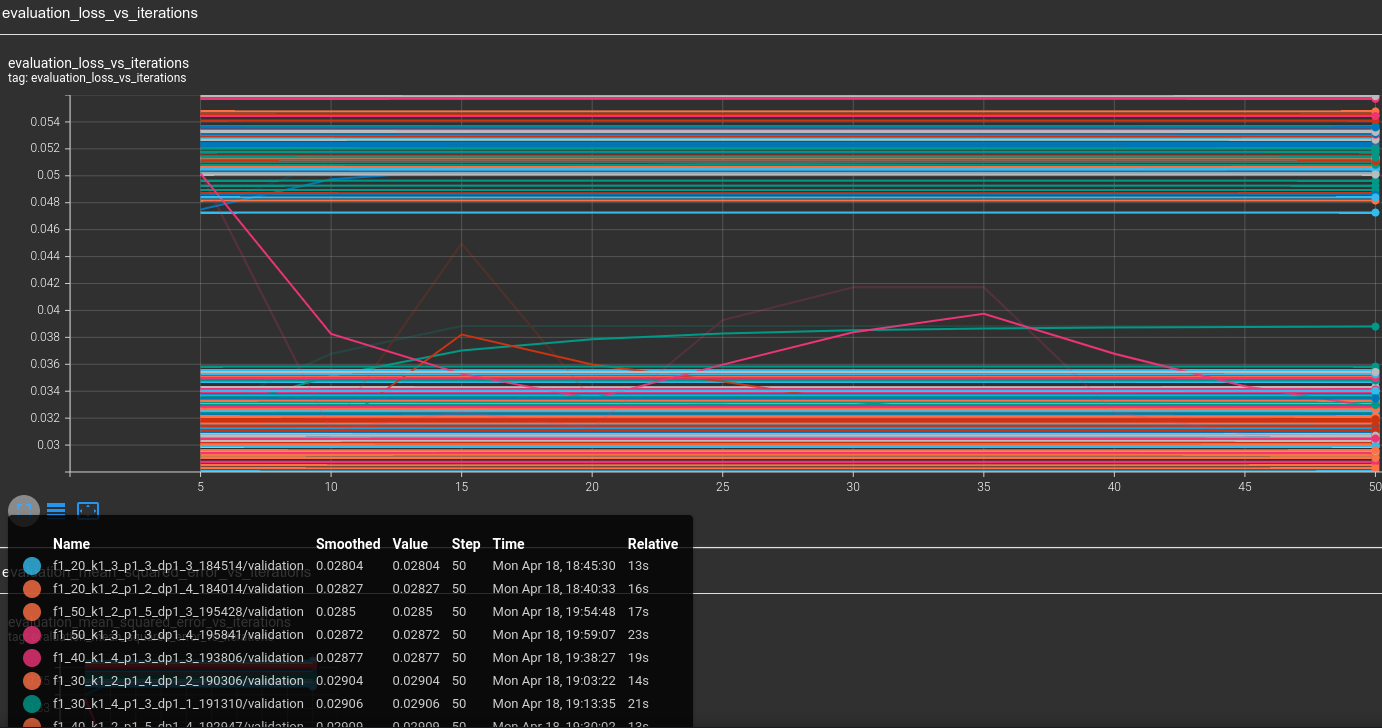
\includegraphics[keepaspectratio, width=\columnwidth]{Screenshot_2022-04-20_23-15-30.png}
    \caption{first run of best validation cases}
    \label{img:1best_cases}
\end{figure}

\begin{figure}[H]
    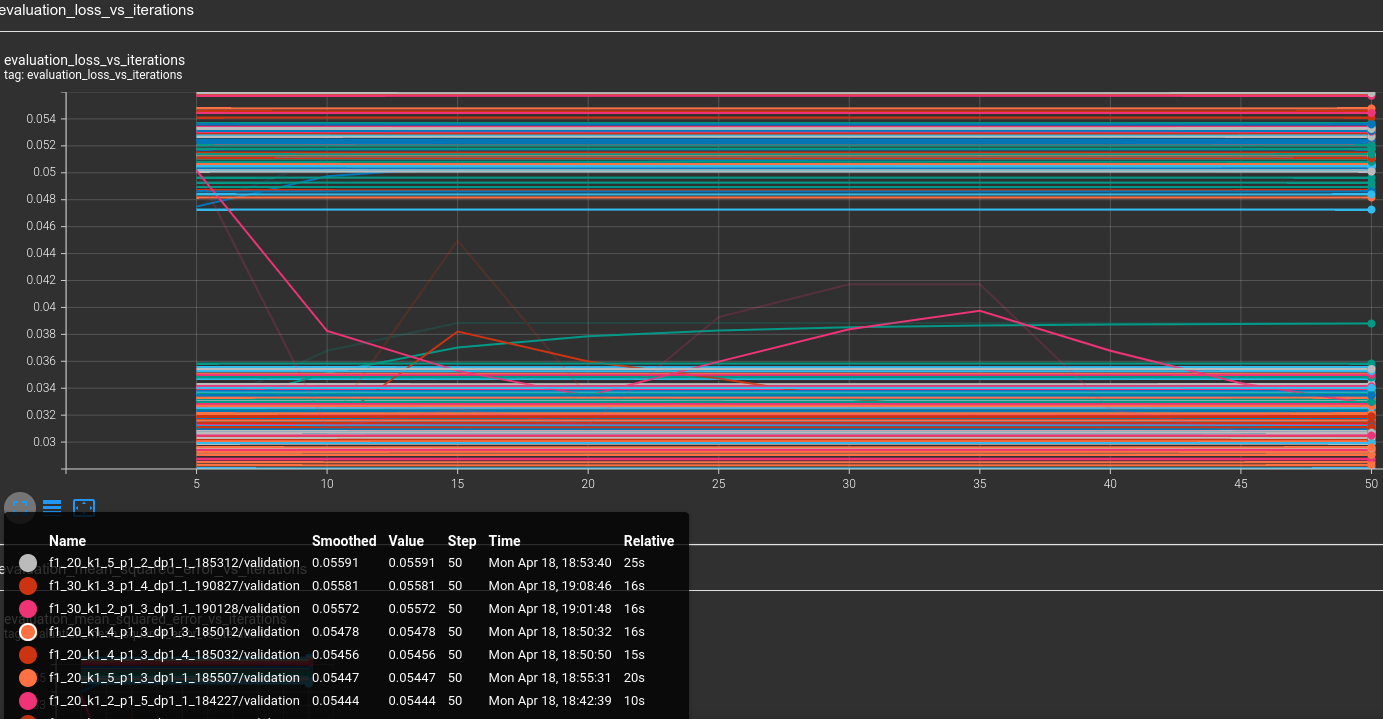
\includegraphics[keepaspectratio, width=\columnwidth]{Screenshot_2022-04-20_23-20-48.png}
    \caption{first run of worst validation cases}
    \label{img:1worst_cases}
\end{figure}


The least performant models \ref{img:1worst_cases} showed that the dropout of 0.1 was too little and that kernels of sizes 4 and 5 were too big.


\begin{figure}[H]
    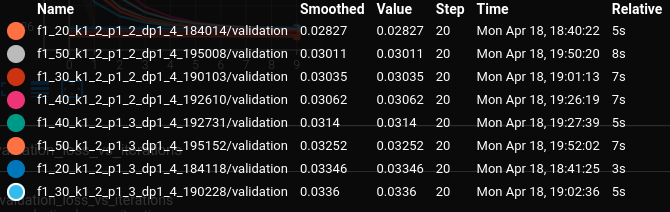
\includegraphics[keepaspectratio, width=\columnwidth]{Screenshot_2022-04-20_23-36-21.png}
    \caption{Final set selected}
    \label{img:final_set}
\end{figure}

Following analysing the first run conclusions, the next step was to create a regex mask that, by trial and error, filtered out the least performant models down to the eight best ones \ref{img:final_set}. The regex selected a dropout rate of 0.4, a kernel of size two and a pooling of sizes 2 and 3.




\section{Performance evaluation}

The testing determined that the best convolution layer for the image processing has 20 filters, a kernel and pooling layer of size two and a dropout rate of 0.4, based on the final filtering and ascending ordering \ref{img:final_set}.




\chapter{Conclusion}



\section{Main achievements}

The main goal of this project was to create a free- and open-source modular and generic library that collects data from image data. This is an arduous task packed with very unexpected obstacles regardless of the extensive research and development. Despite the obstacles faced, the current work lays the foundations and infrastructure for such a system.


The object detection and tracking system have performed well, considering the difficult task of tracking a very dynamic environment. The algorithm is neat to fulfil the goal and can it improved and extended over time. Although it does not have perfect accuracy (and is expected to improve over time), other future components will be developed to work on the limits of this module.


The dataset generation module is probably the most exciting module because it circumvents the current dataset limitation and allows for great flexibility. This allows new possibilities to train a wide range of different machine learning models.


The most significant achievement was the development of an end-to-end data collection infrastructure that is robust and has the potential to be used for a relevant problem in the real world. It was planned and designed toward what the industry and academia are looking for, and it is for everyone to use, modify, improve and redistribute without any limits.


In all, it is safe to assume that a significant amount of the proposed initial objectives were accomplished. The remaining objectives were also addressed but may need more research and work to be accomplished as they generally pose significant technical challenges.


\section{Main limitations of work}


This project accomplished most of its goals, but many aspects are not achievable, at least now. The primary and ultimate limitation is that the output will always be an approximation/estimation of the natural world since it captures data from the analogue world to the digital one. Recognising this irrefutable limitation gives the correct perspective on what is possible and to seek to improve or create. Future development must have these assumptions always present.


The data comes only from the camera view. This fact underlies a relevant limitation. It is impossible to know precisely where players off the camera view are. The position of all players at all times is valuable in football data science projects. The promising solution is to mitigate the issue by developing a spatio-temporal model of players' positions in previous matches. This could be used to estimate where the missing players could be.


Identifying players is essential in sports data science as there is a need to calculate the performance of each individual player. Currently, this solution does not do visual recognition of players as it goes beyond the current goals. However, it will be a priority goal once the solution's basic functionality is completed.


The ball and players will, in the initial stage, be mapped in 2D dimensions. This does not reflect the nature of the sport. The players and the ball have movements in the 3D space (humans jumping and the ball being shot), and it is critical data, especially the ball trajectory in shots, to analyse the expected goals metric. Additionally, the current ball 2D trajectory tracking is also prone to be interrupted whenever an object obstructs the camera view. This is a significant limitation that needs to be addressed as a priority for this solution to be viable. These issues are complex and require special planning to find the most effective approach.




\section{Future work}




The solution has great potential, so there is a long list of future work to fulfil it. An excellent improvement is to parallelise and multithread the current program, which was not done yet because it is still in an experimental phase, and it is not time efficient to invest in applying these techniques to code that may be changed or removed. The performance improvement will be implemented once the program reaches a good level of efficacy. Additionally, the execution, training and testing of the many modules of the solution have been done solely on a local machine that cannot run as fast as a system like this should. For this reason, the code should be moved to a cloud platform so that it increases the performance drastically.


The more general improvements that could add immediate value are improving the image processing and the detection/tracking system to work with low-quality recordings resulting from terrible weather conditions or inadequate lighting conditions. Besides that, the system uses a bitwise "and" to apply a green mask to the video, but not all pitches are green. This could be solved by letting the operator choose the "masking colour" for pitches that do not have green grass or if the pitch is snowy.


An essential component of sports data science is to evaluate the performance of each individual, and that is only possible if each player is identified when the data is being collected. The identification could first start by using the numbers on shirts to identify players so that an additional model could then learn the visual characteristics (body visuals and boots) and then predict the players when the numbers are not visible by their visuals. In this case, the referees should be filtered by their kit colour because the team of officials always has a different colour.


In the first runs of the human detection algorithm, a bug emerged that detected a massive sized human detection. This is a bug, but it was not fixed because a neat algorithm was not found to this moment that could filter it in a consistent matter. Different recordings will have to produce different bounding boxes, so choosing a fixed threshold to filter is not wise. The solution should calculate all human detections' median and standard deviation before filtering the outcasts.


Any team sport is dynamic, meaning that a match has many plays (defined as segments of the match, segmented by set-pieces), and the video stream has regularly replays or sudden angles changes. The system should process these events. These segments should be dealt with manually (following the development strategy) by giving the operator control of segmentation. The final solution should be an unsupervised clustering machine learning model that processes a stream of images to detect these segmentations.


Data generation has a significant problem if the camera frame points beyond the horizon in the 3D model. This is important because minor stadiums have lower stands so that camera angles will be pointing higher than in bigger stadiums. It is necessary to return an inner segment to detect the geometric reconstruction. In this issue, the solution may be approximating somehow the inner section to a reasonable and workable value. The dataset generation could also improve by adding noise to the images in the dataset to emulate a real-world scenario.


The solution's data collection is expected to be chaotic due to the intermittent nature of object detection, object tracking, and geometric distortion. This is a serious issue that can only be solved by creating a spatio-temporal data stream correction to smooth and generally fix inconsistencies in the data output.


The nature of collective sports is a set of relationships between individual players. The sport, as a function, can be reasoned based on its spatio-temporal states. This definition of sports can entail that a logical programming language and/or logical reasoner could be helpful if applied to it. As such, outputting the data as an ontology could be promising for sports data science.


Human pose estimation is a fascinating technique that could be very insightful in analysing players' body performance and language. It would enrich the data to give much more context to the analysis, primarily if it could be used to train an action predicting model. A few datasets of past matches containing a match's event stream (passes, shots, tackles, etc.) could be used to undertake extrapolation and predict many types of actions with outstanding accuracy, at least in theory.


The most remarkable future improvement could be the integration of a 3D simulation environment which can be used to enhance the current capabilities firstly and additionally add extra functions that could take this project to the next level as another source of synthetic data which could be complementary to the existing blender generation dataset environment. The Google Research Football Environment \cite{gfootball_env} is a former open-source football computer game that Google's Artificial intelligence department repurposed to test and train AI adversary models in a highly stochastic environment. The project has been successful, and it was used in many different AI events and competitions. Humans can control it, but the ultimate goal is for each team/player to be controlled by an intelligent agent in a realistic 3D physical environment that generates 3D positional data of all objects on the pitch. After training these models, the teams play against each other and generate essential data to evaluate the models' performance. This final output data, along with the corresponding visual data recorded, could be used to improve the training/validation/testing of the existing machine learning models for object and geometric detection models since the data collected intersect the one generated on Blender. Although promising, the real value is to use the in-game simulator to extract data that signals actions undertaken by players, 3D player pose estimation, objects 3D trajectory, in-game play segments and set-piece recognition. These additional features are precious to increase the data points and enrich the data, which contributes to automating, even more, some manual operations that the operator performs. It is also conceivable to create an extra model that corrects players tracking (to smooth it out) and even augments the off-screen player positions (by combining spatio-temporal in-game data), which is genuinely groundbreaking. Predicting the off-screen players' position is critical because it mitigates one of the most significant limitations of this approach of using regular match streams.


The Google Football environment \cite{gfootball_env} is specific to football which is contrary to the objective of being a general solution for any sports. The long term solution is to create a free- and open-source modular game environment to simulate other sports and even be used as bases for standalone sports games. This proposal is far-fetched as it is a whole other project, but it is a sustainable project to leverage sports data science and gaming development. For these reasons, this could be added to the community's long term roadmap.



\printbibliography



\appendix
\renewcommand{\thesection}{\Alph{section}.\arabic{section}}
\setcounter{section}{0}
\begin{appendices}


\section{Images}


\subsection{Results section}

\begin{figure}[H]
    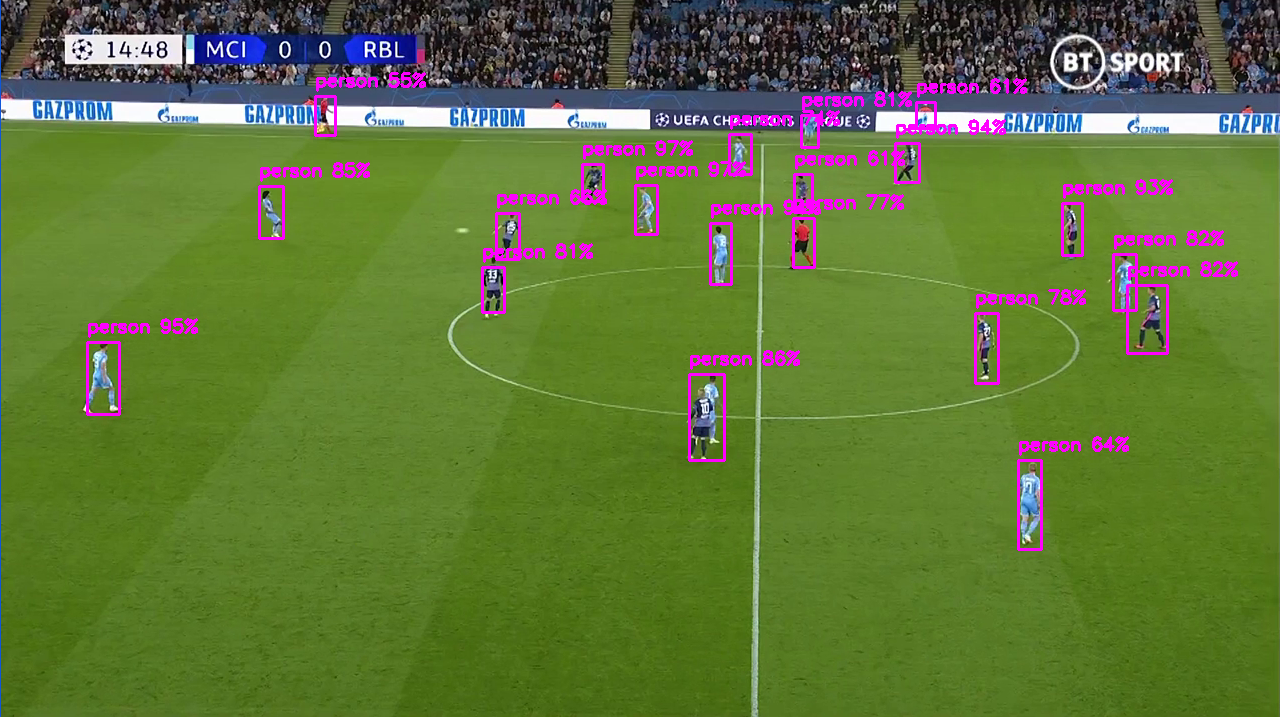
\includegraphics[keepaspectratio, width=\columnwidth]{first.png}
    \caption{First detection, no ball detected}
    \label{img:1}
\end{figure}
\begin{figure}[H]
    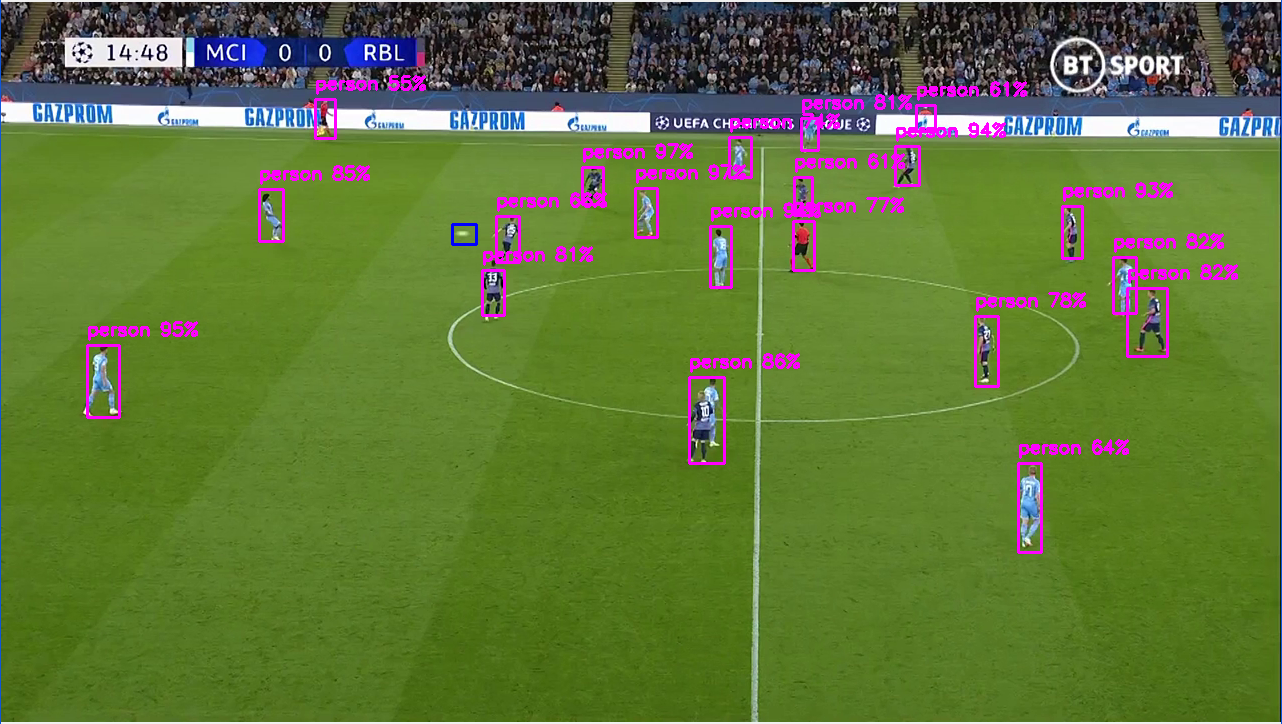
\includegraphics[keepaspectratio, width=\columnwidth]{Screenshot_2022-03-03_21-32-51.png}
    \caption{Manually labelling ball}
    \label{img:2}
\end{figure}
\begin{figure}[H]
    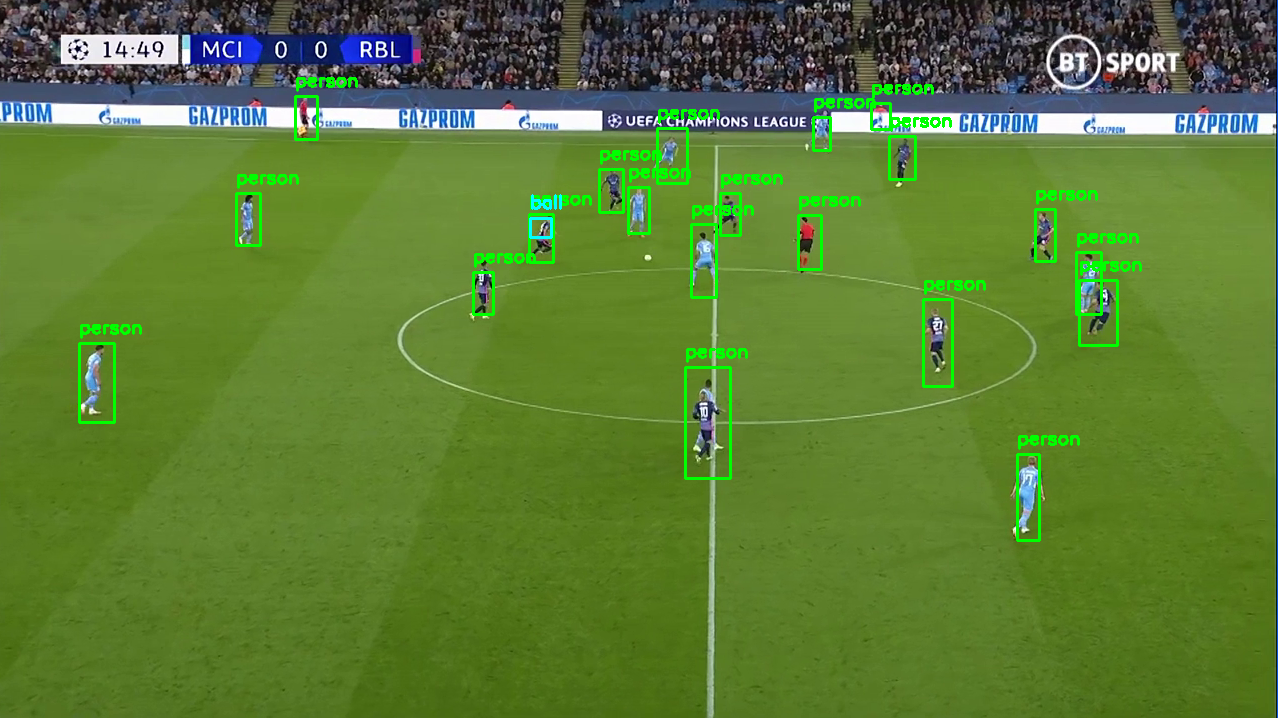
\includegraphics[keepaspectratio, width=\columnwidth]{Screenshot_2022-03-03_21-35-39.png}
    \caption{Ball tracking error}
    \label{img:3}
\end{figure}
\begin{figure}[H]
    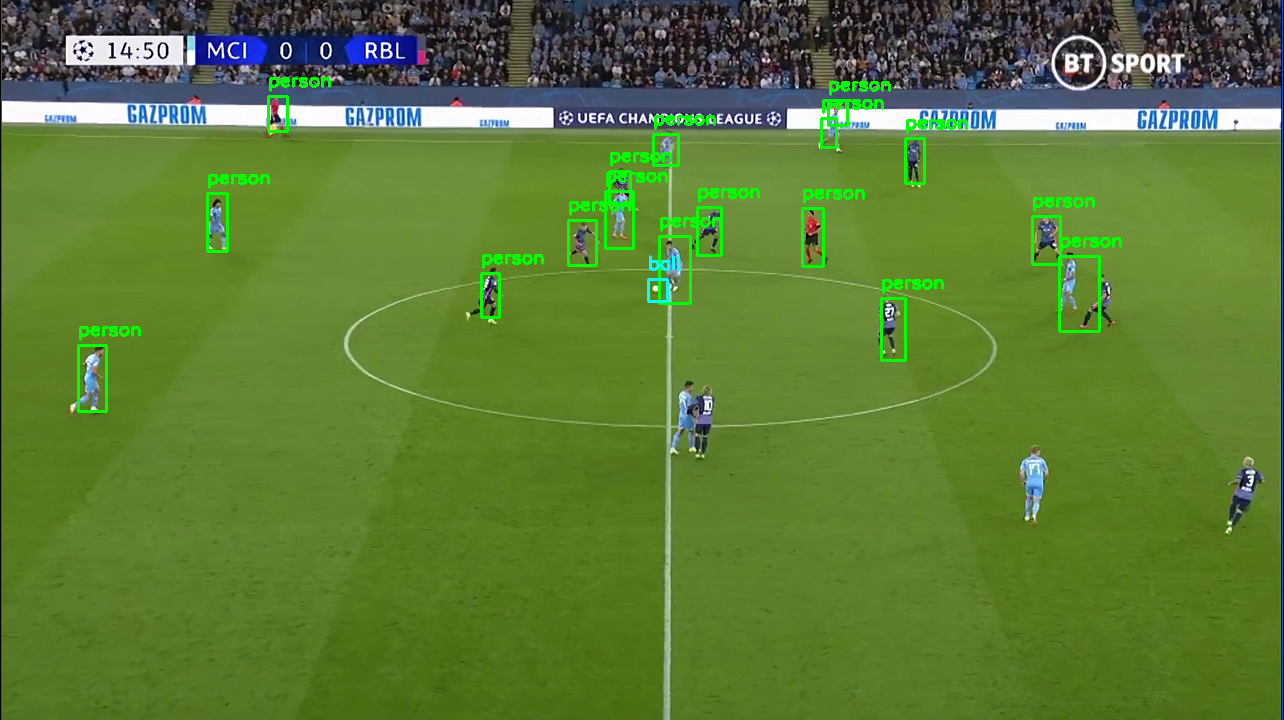
\includegraphics[keepaspectratio, width=\columnwidth]{Screenshot_2022-03-03_21-36-05.png}
    \caption{New players on screen are not detected}
    \label{img:4}
\end{figure}
\begin{figure}[H]
    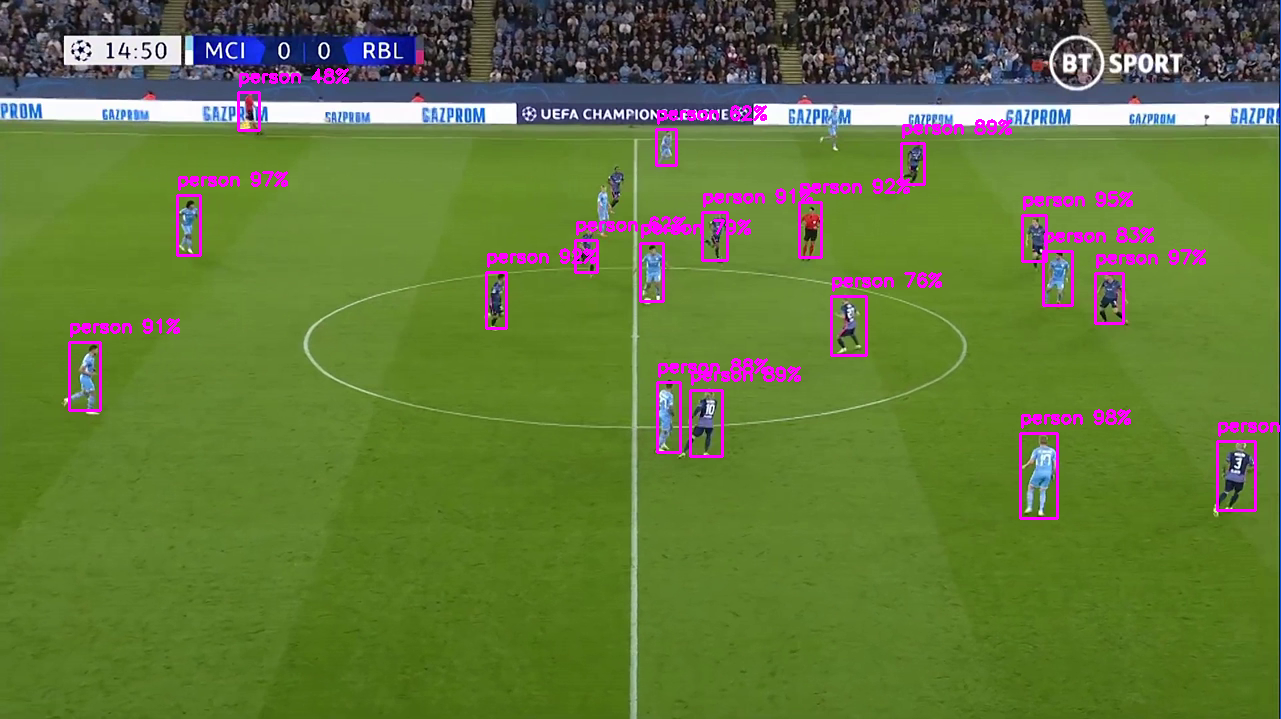
\includegraphics[keepaspectratio, width=\columnwidth]{Screenshot_2022-03-03_21-38-04.png}
    \caption{Ball tracking lost}
    \label{img:5}
\end{figure}
\begin{figure}[H]
    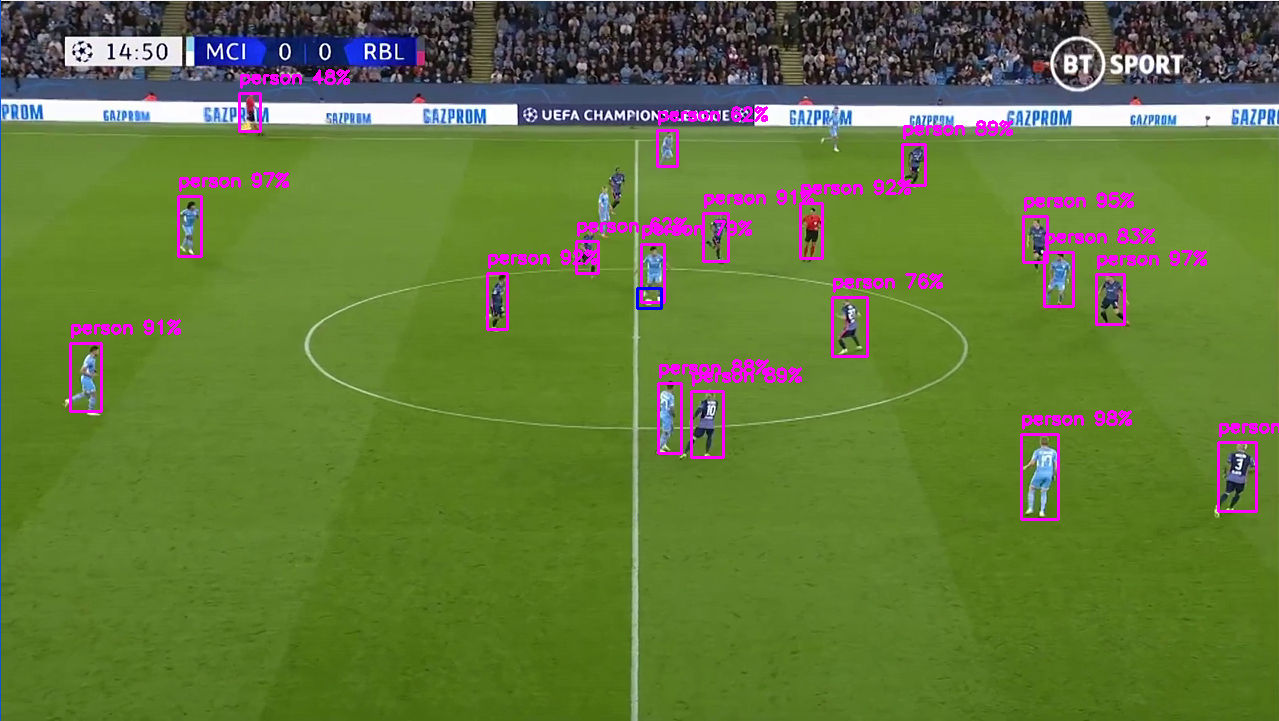
\includegraphics[keepaspectratio, width=\columnwidth]{Screenshot_2022-03-03_21-36-47.png}
    \caption{New ball labelling}
    \label{img:6}
\end{figure}
\begin{figure}[H]
    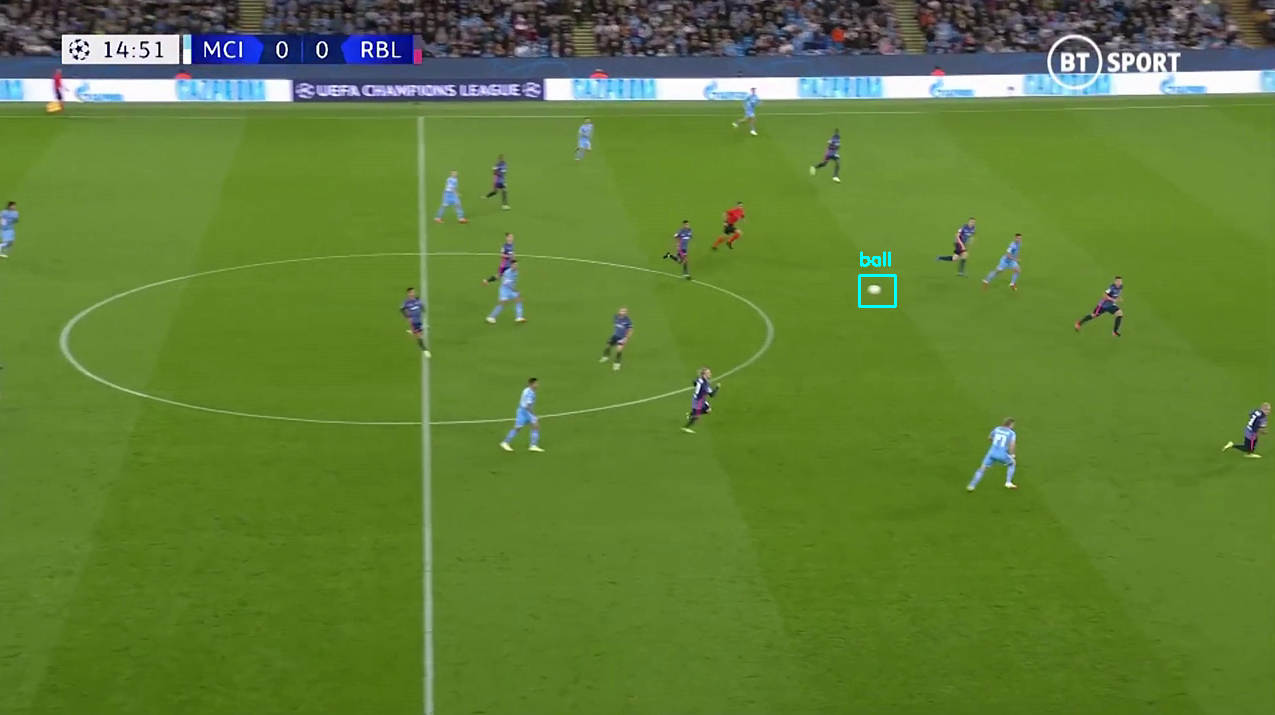
\includegraphics[keepaspectratio, width=\columnwidth]{Screenshot_2022-03-03_23-05-49.png}
    \caption{Ball tracking running, some players go off screen and tracking lost}
    \label{img:7}
\end{figure}
\begin{figure}[H]
    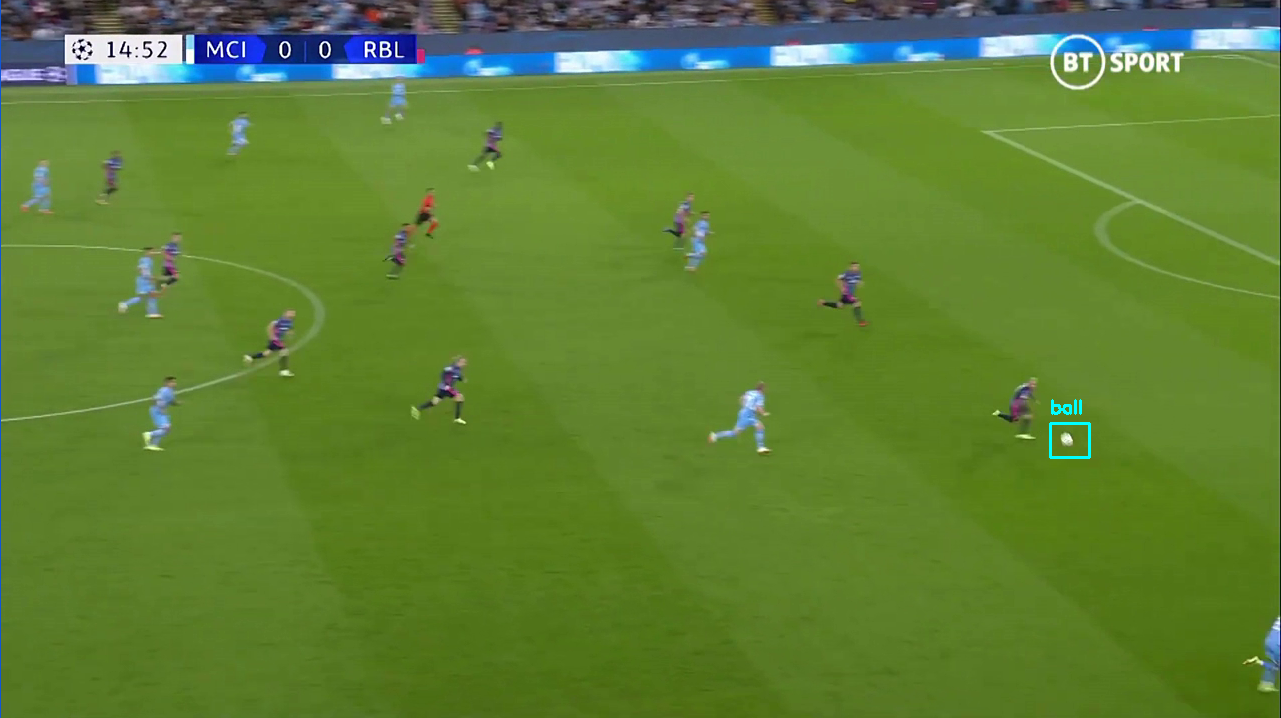
\includegraphics[keepaspectratio, width=\columnwidth]{Screenshot_2022-03-03_23-06-03.png}
    \caption{Player's tracking is lost again, ball tracking continues}
    \label{img:8}
\end{figure}
\begin{figure}[H]
    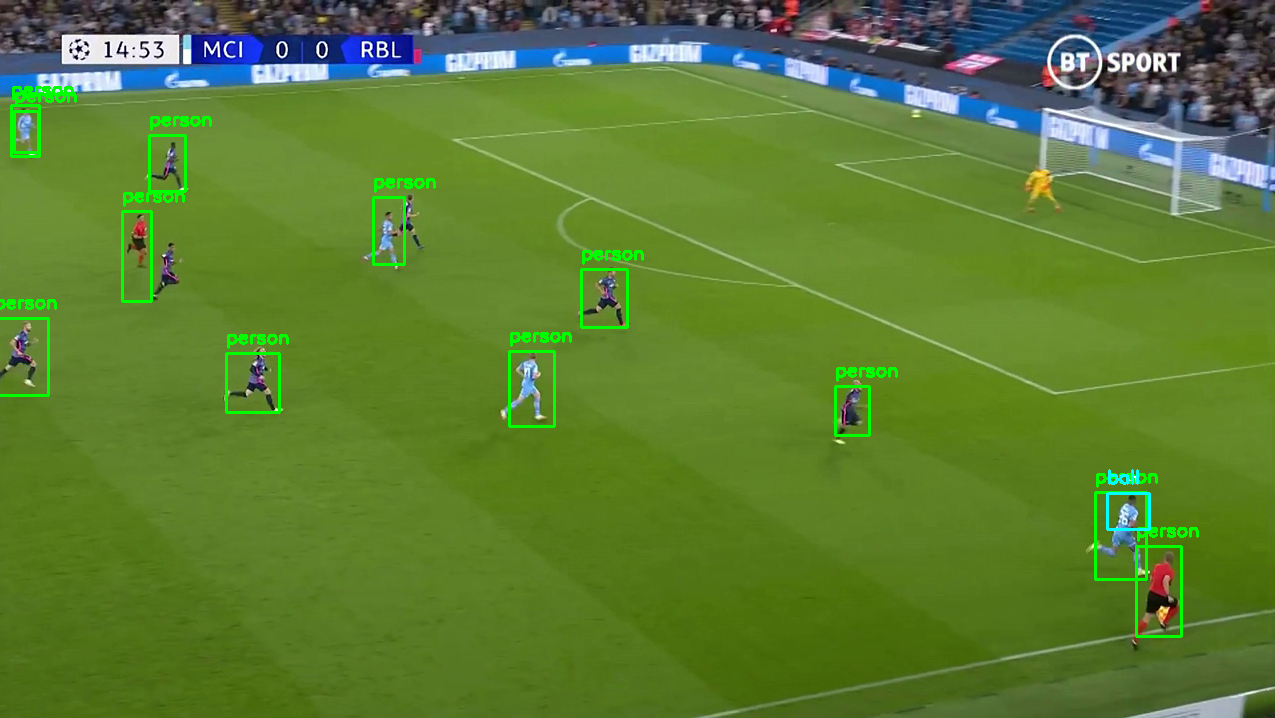
\includegraphics[keepaspectratio, width=\columnwidth]{Screenshot_2022-03-03_23-06-18.png}
    \caption{Players is running but some players are not detected, ball tracking is wrong}
    \label{img:9}
\end{figure}
\begin{figure}[H]
    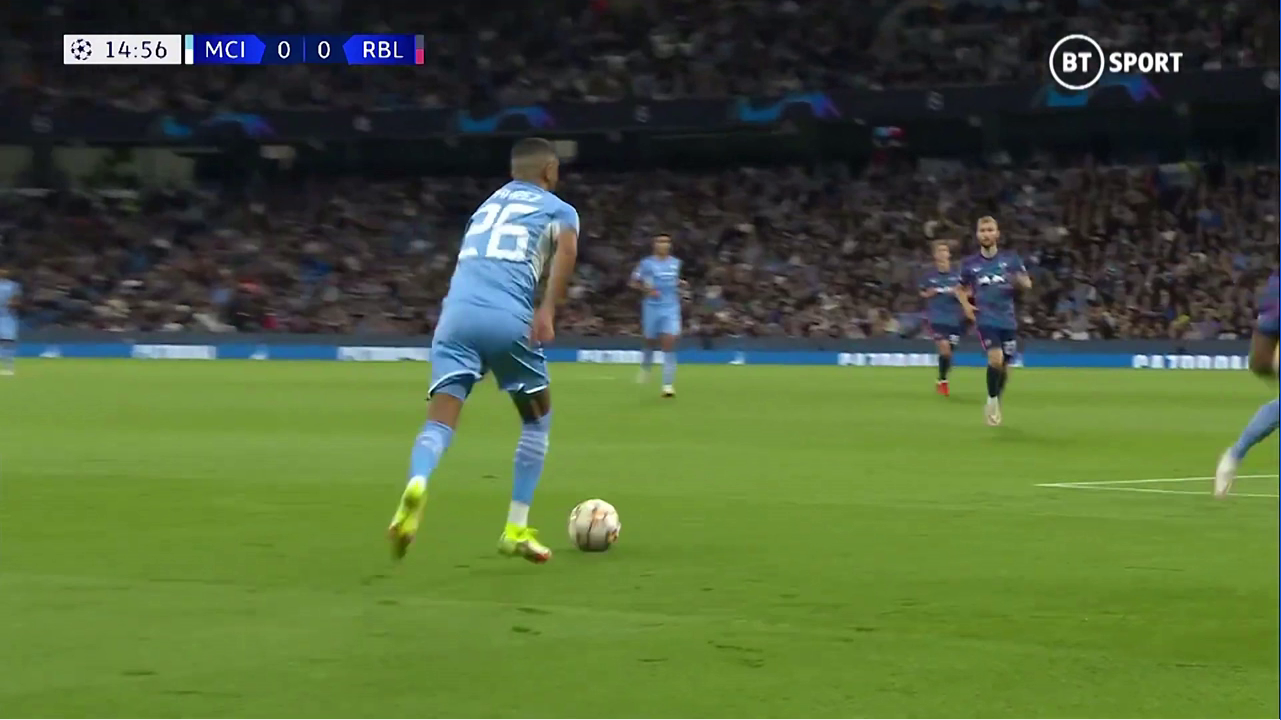
\includegraphics[keepaspectratio, width=\columnwidth]{Screenshot_2022-03-03_21-39-53.png}
    \caption{Different camera angle}
    \label{img:10}
\end{figure}
\begin{figure}[H]
    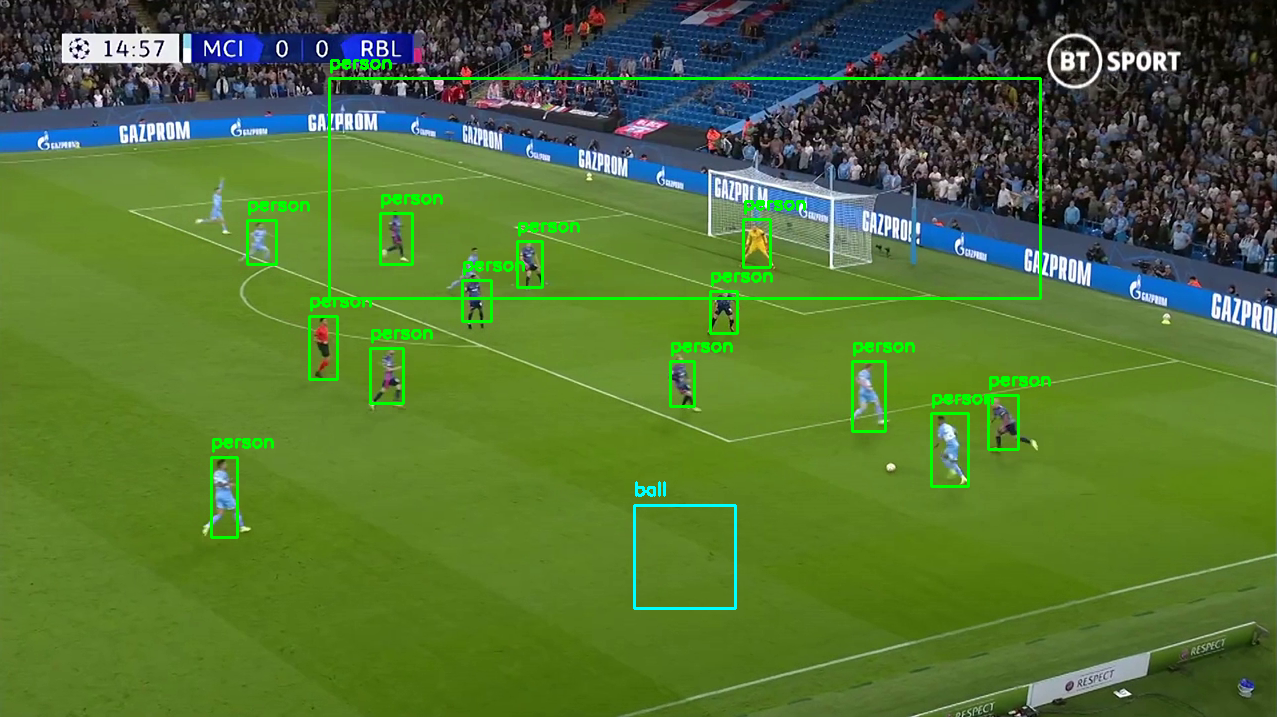
\includegraphics[keepaspectratio, width=\columnwidth]{Screenshot_2022-03-03_23-06-43.png}
    \caption{One wrong human detection and ball detection is wrong as well}
    \label{img:11}
\end{figure}
\begin{figure}[H]
    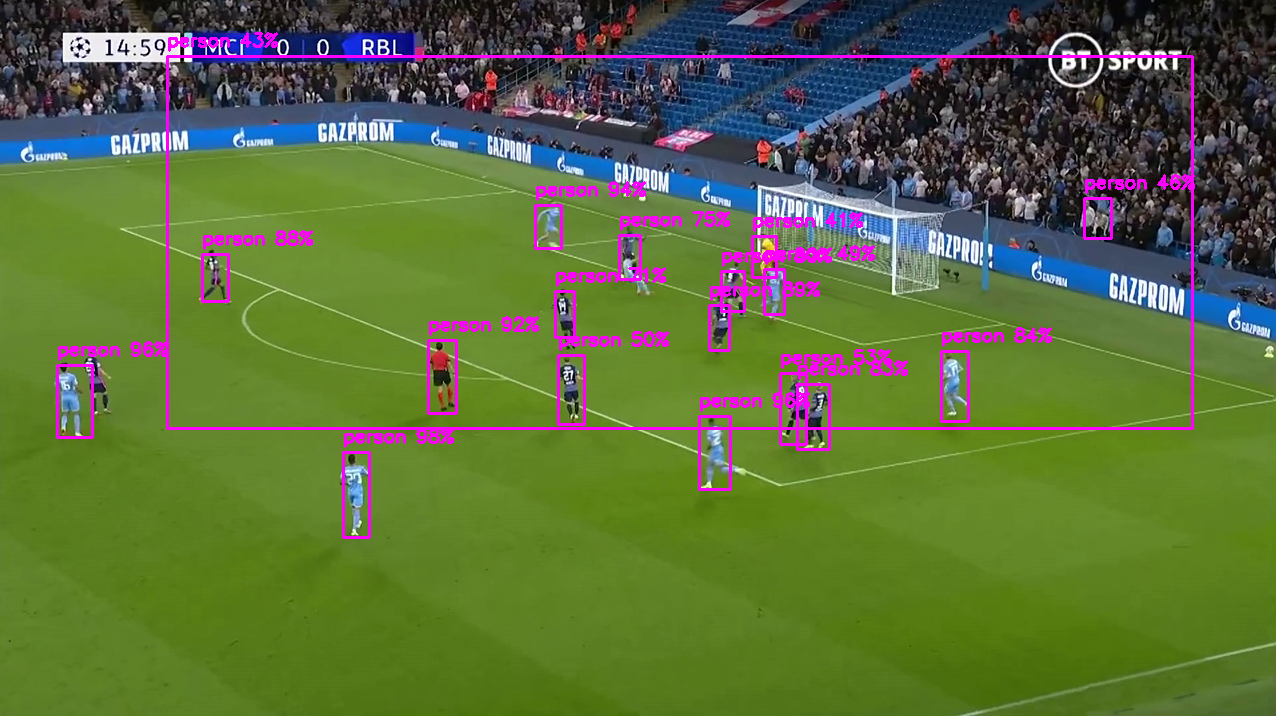
\includegraphics[keepaspectratio, width=\columnwidth]{Screenshot_2022-03-03_23-08-00.png}
    \caption{Detection bug continues, fan is detected and ball tracking is lost}
    \label{img:12}
\end{figure}
\begin{figure}[H]
    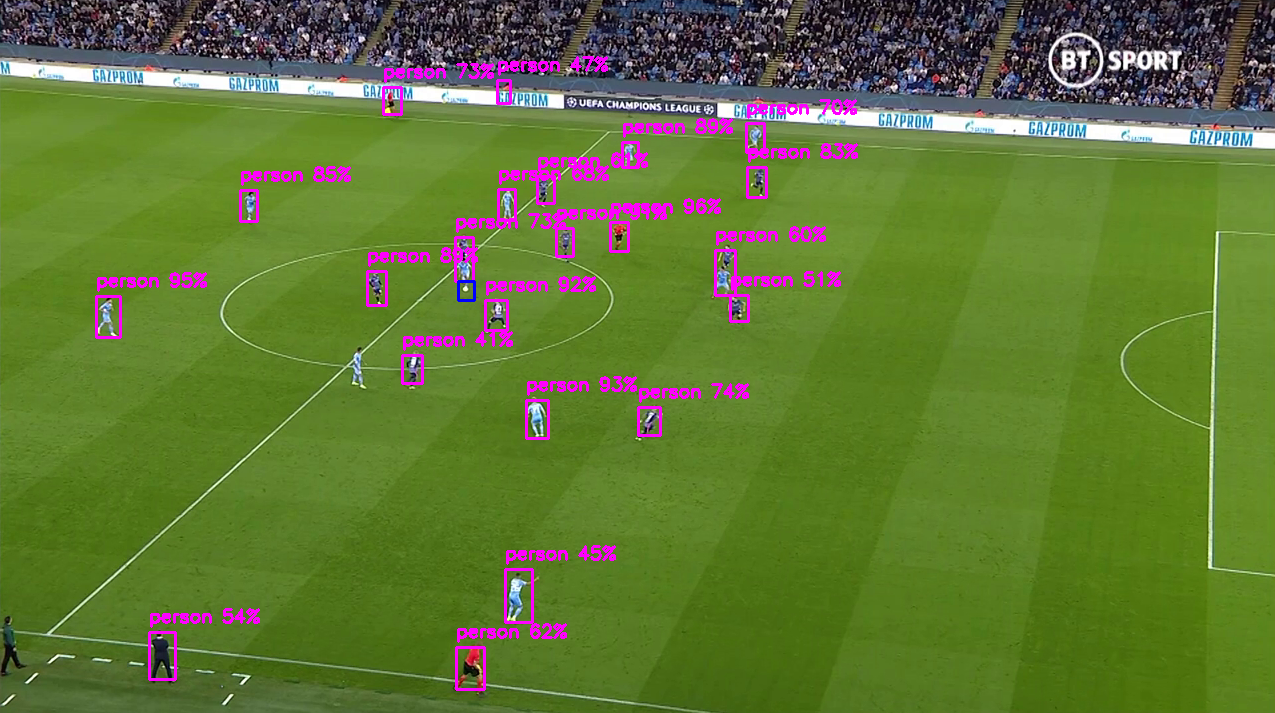
\includegraphics[keepaspectratio, width=\columnwidth]{Screenshot_2022-03-03_23-09-45.png}
    \caption{New perspective, players were detected and ball is being labelled}
    \label{img:13}
\end{figure}
\begin{figure}[H]
    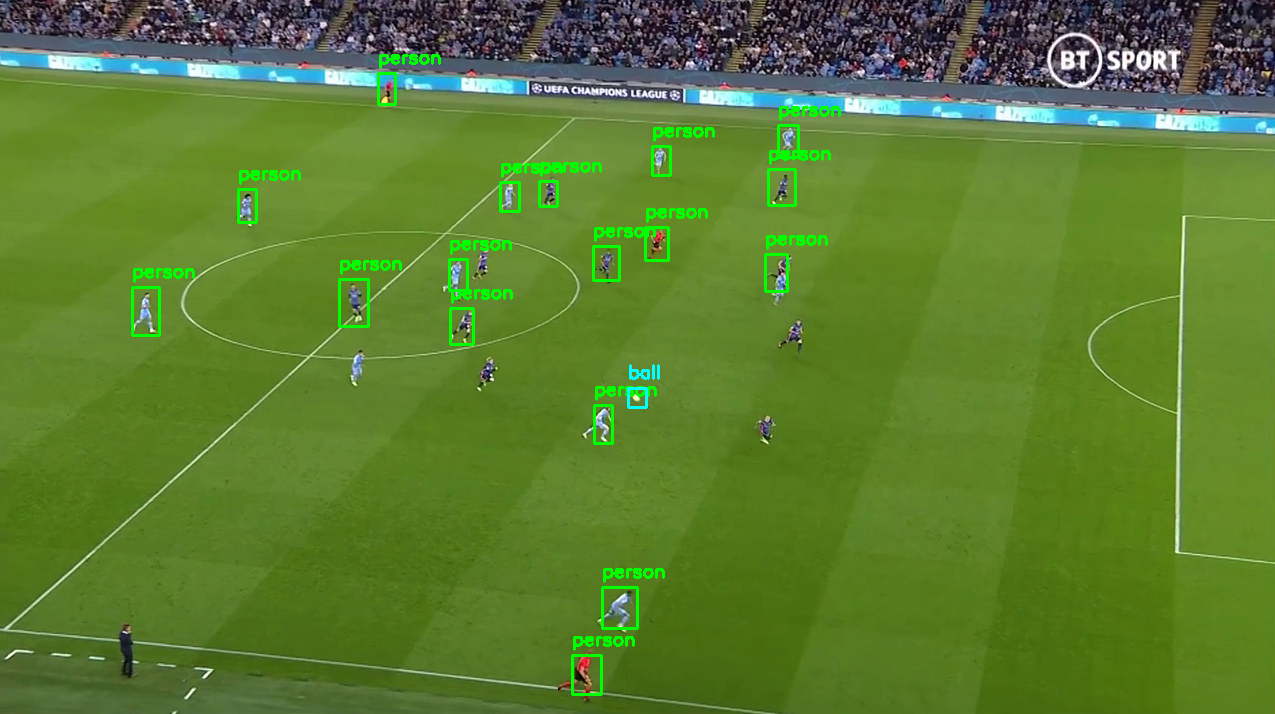
\includegraphics[keepaspectratio, width=\columnwidth]{Screenshot_2022-03-03_23-10-58.png}
    \caption{New perspective, players and ball are being tracked}
    \label{img:14}
\end{figure}
\begin{figure}[H]
    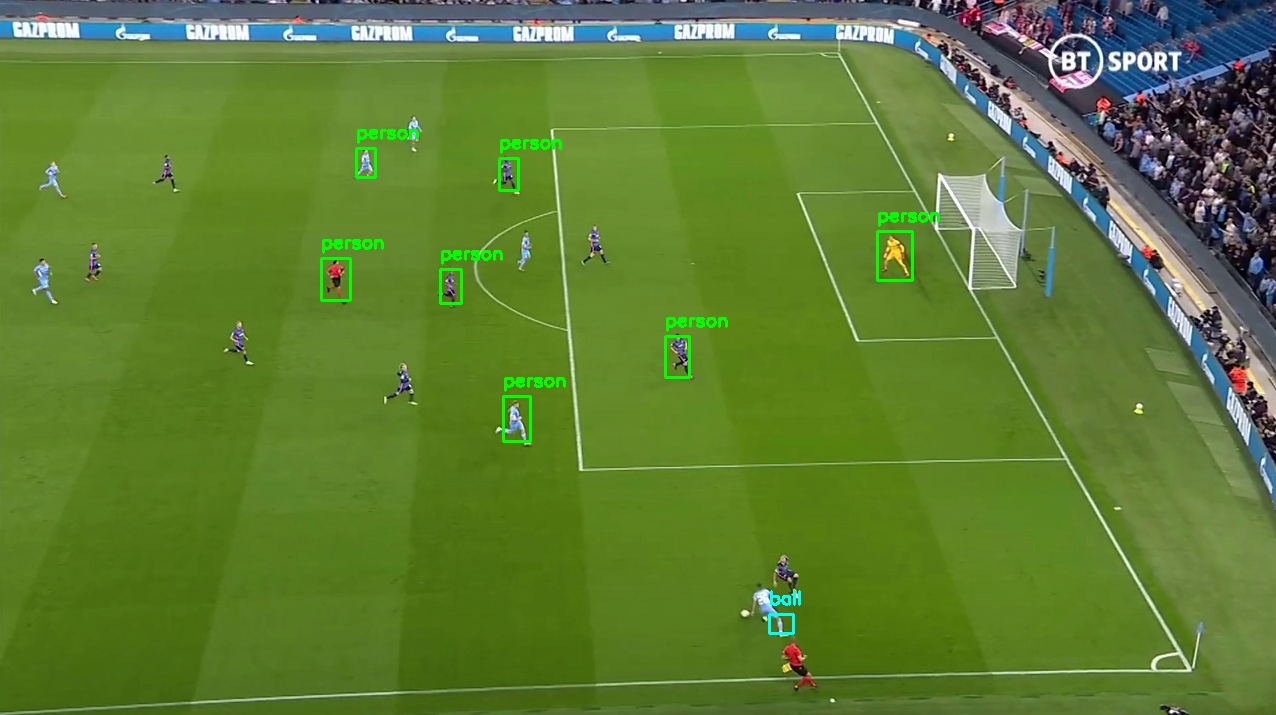
\includegraphics[keepaspectratio, width=\columnwidth]{Screenshot_2022-03-03_23-12-29.png}
    \caption{Yet another perspective, most players detected but ball tracking is wrong}
    \label{img:15}
\end{figure}
\begin{figure}[H]
    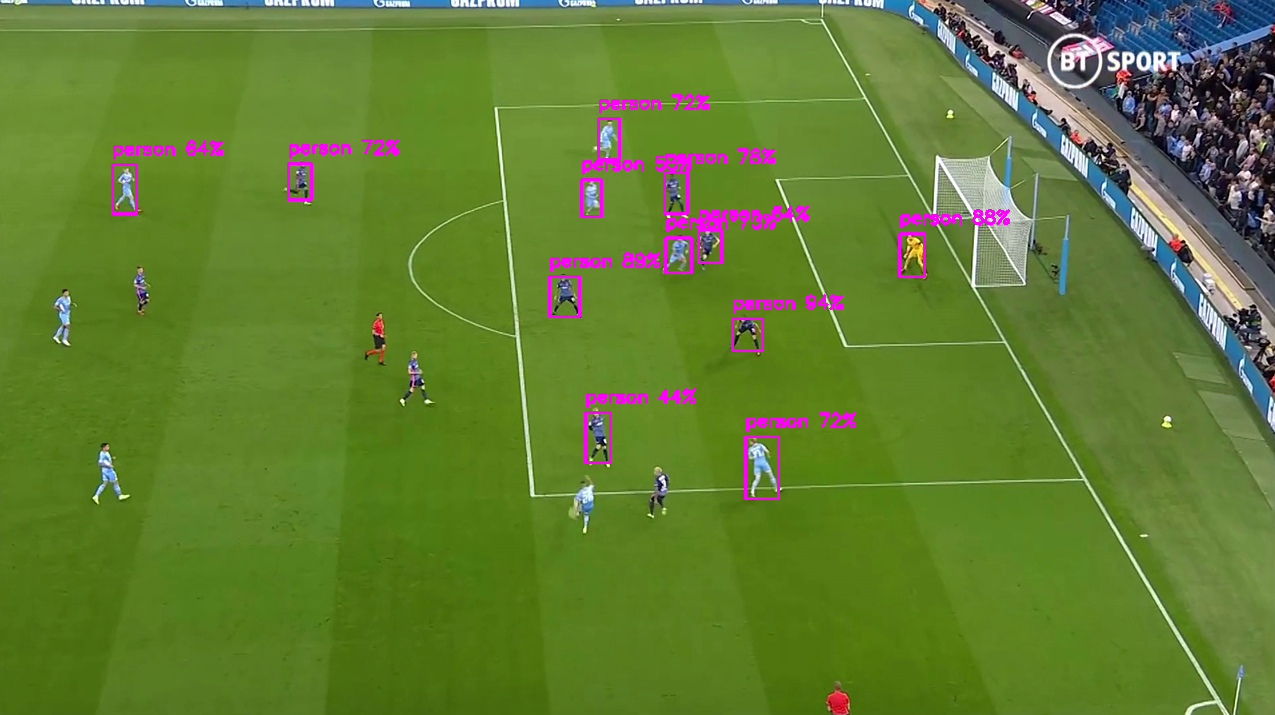
\includegraphics[keepaspectratio, width=\columnwidth]{Screenshot_2022-03-03_23-13-18.png}
    \caption{Half of players are detected, all in the most important zone}
    \label{img:16}
\end{figure}



\subsection{3D Modelling}



\begin{figure}[H]
    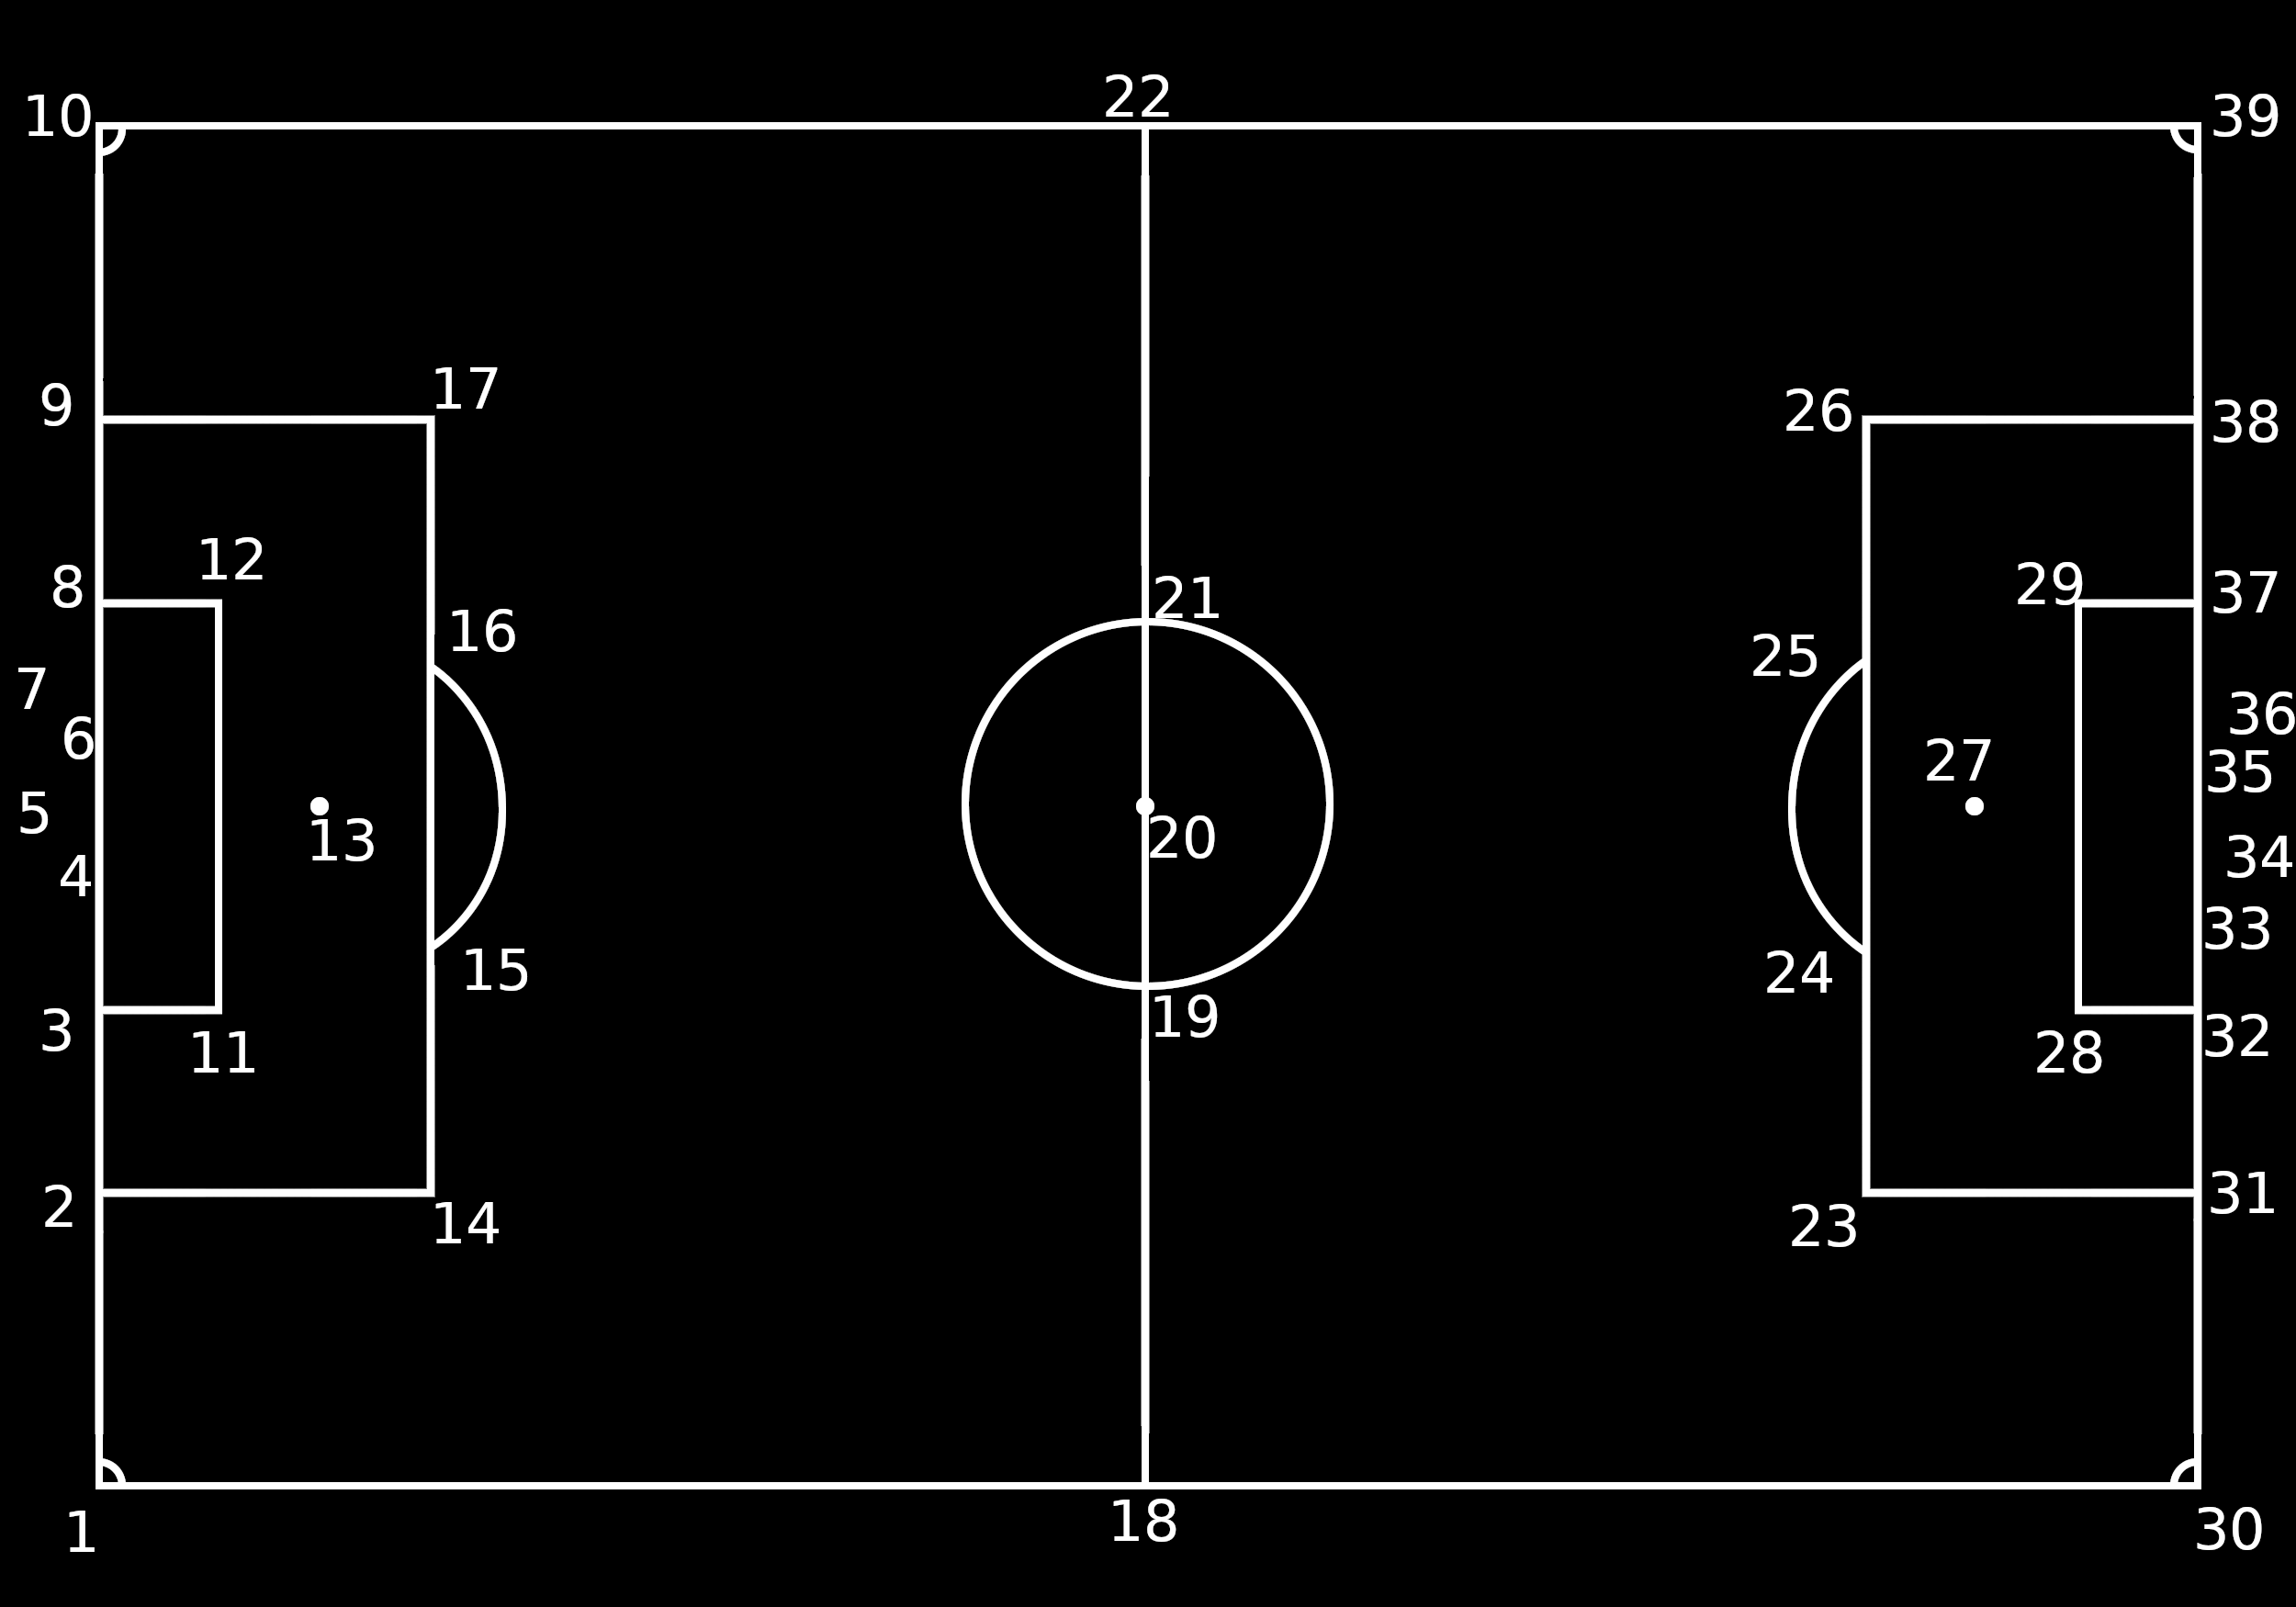
\includegraphics[keepaspectratio, width=\columnwidth]{coordinates.png}
    \caption{Reference Map}
    \label{img:ref_map}
\end{figure}

\begin{figure}[H]
    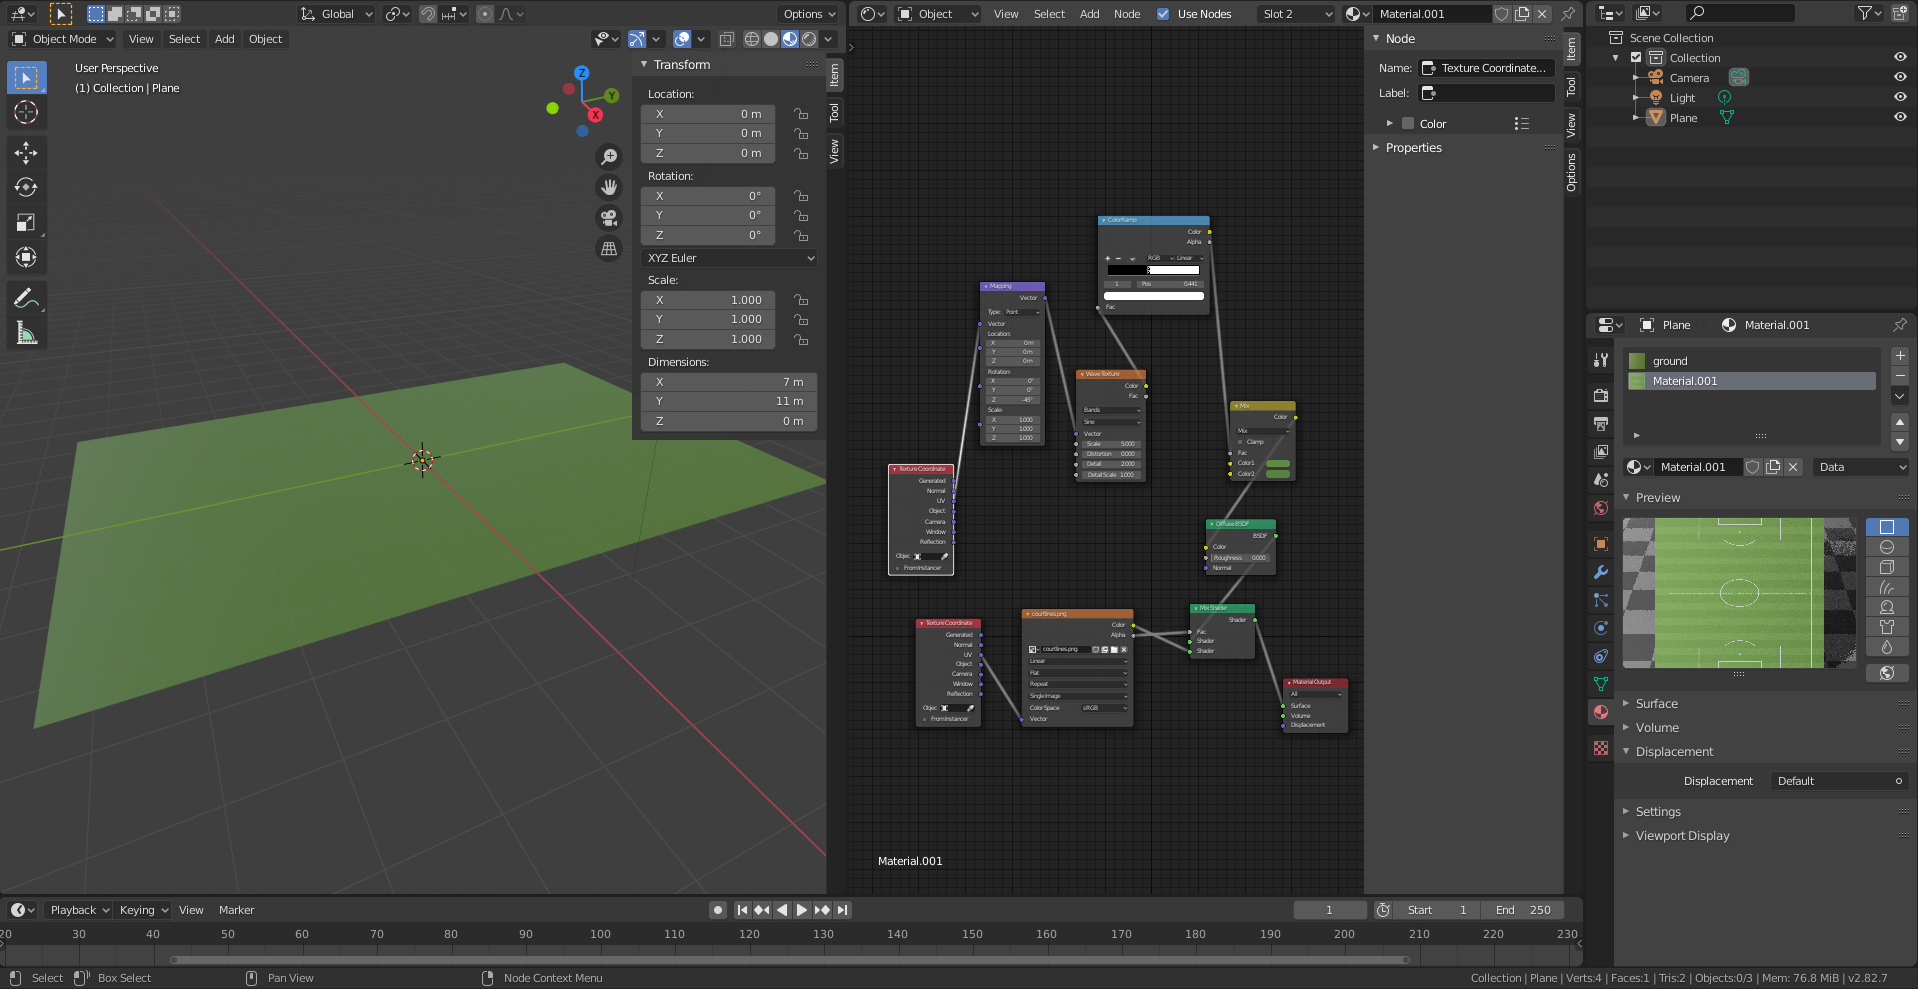
\includegraphics[keepaspectratio, width=\columnwidth]{Screenshot_from_2021-10-22_13-59-52.png}
    \caption{Development of 3D blender model}
    \label{img:texture}
\end{figure}


\begin{figure}[H]
    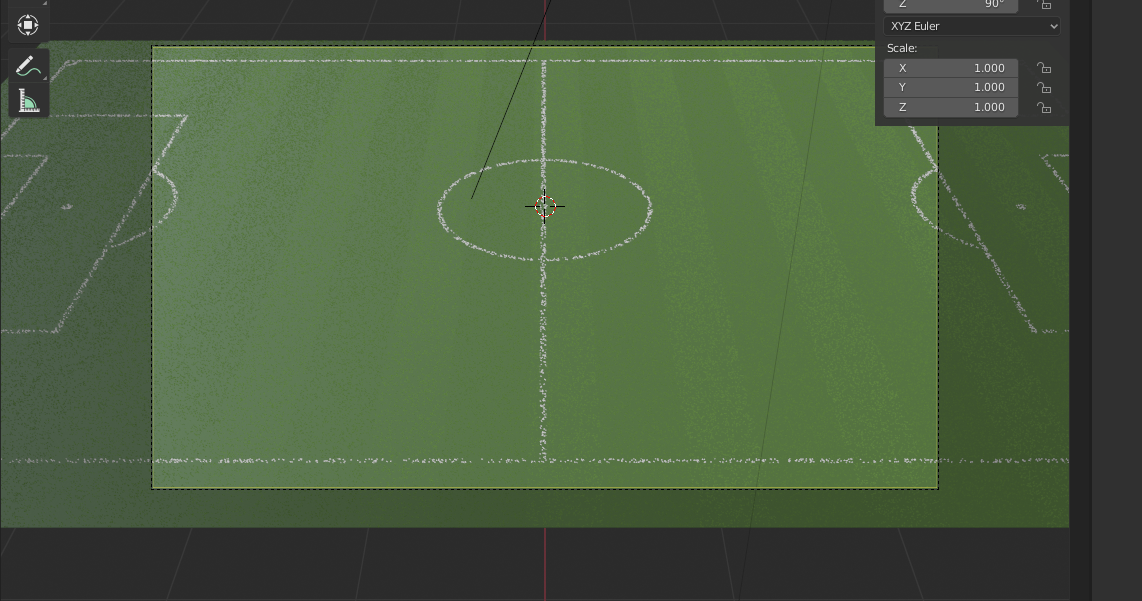
\includegraphics[keepaspectratio, width=\columnwidth]{Screenshot_2021-12-17_19-08-06.png}
    \caption{Camera view in blender}
    \label{img:cam_grass}
\end{figure}


\begin{figure}[H]
    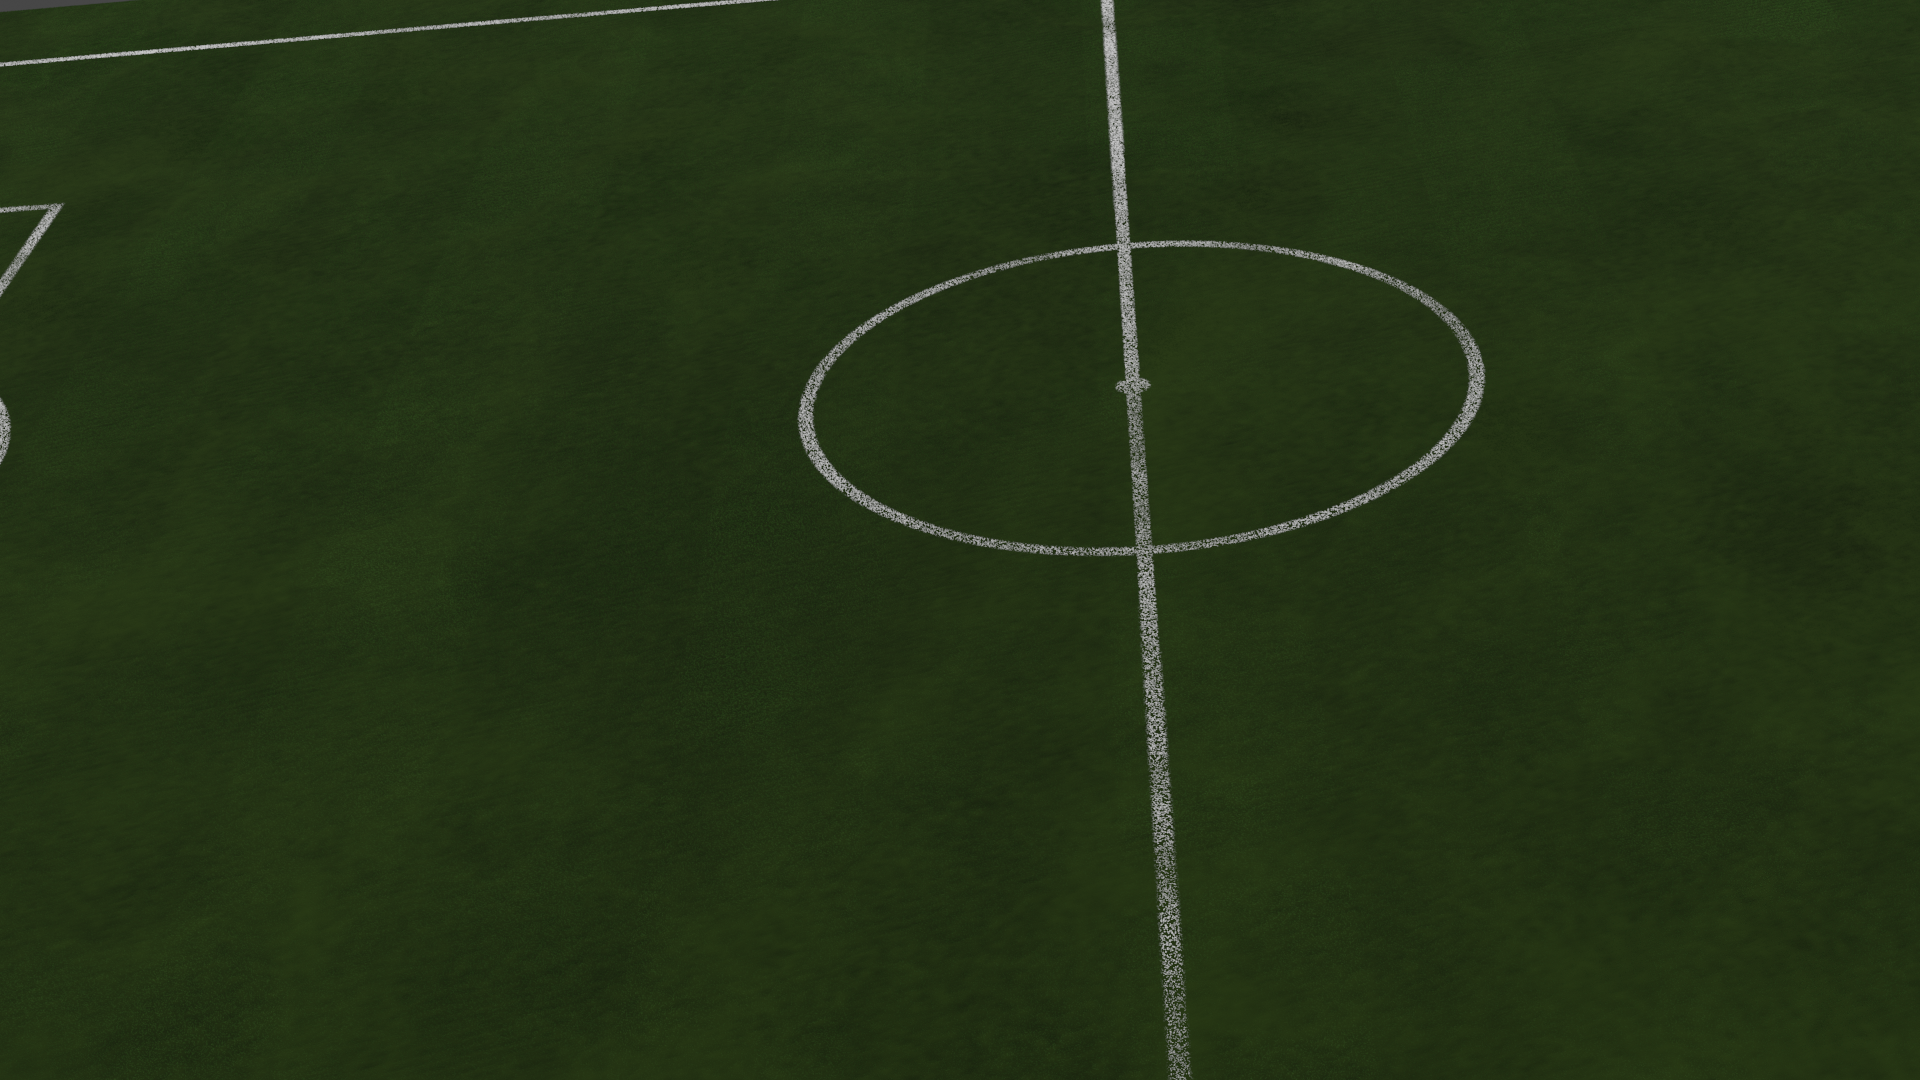
\includegraphics[keepaspectratio, width=\columnwidth]{image.png}
    \caption{Camera rendered image}
    \label{img:camera_view}
\end{figure}


\begin{figure}[H]
    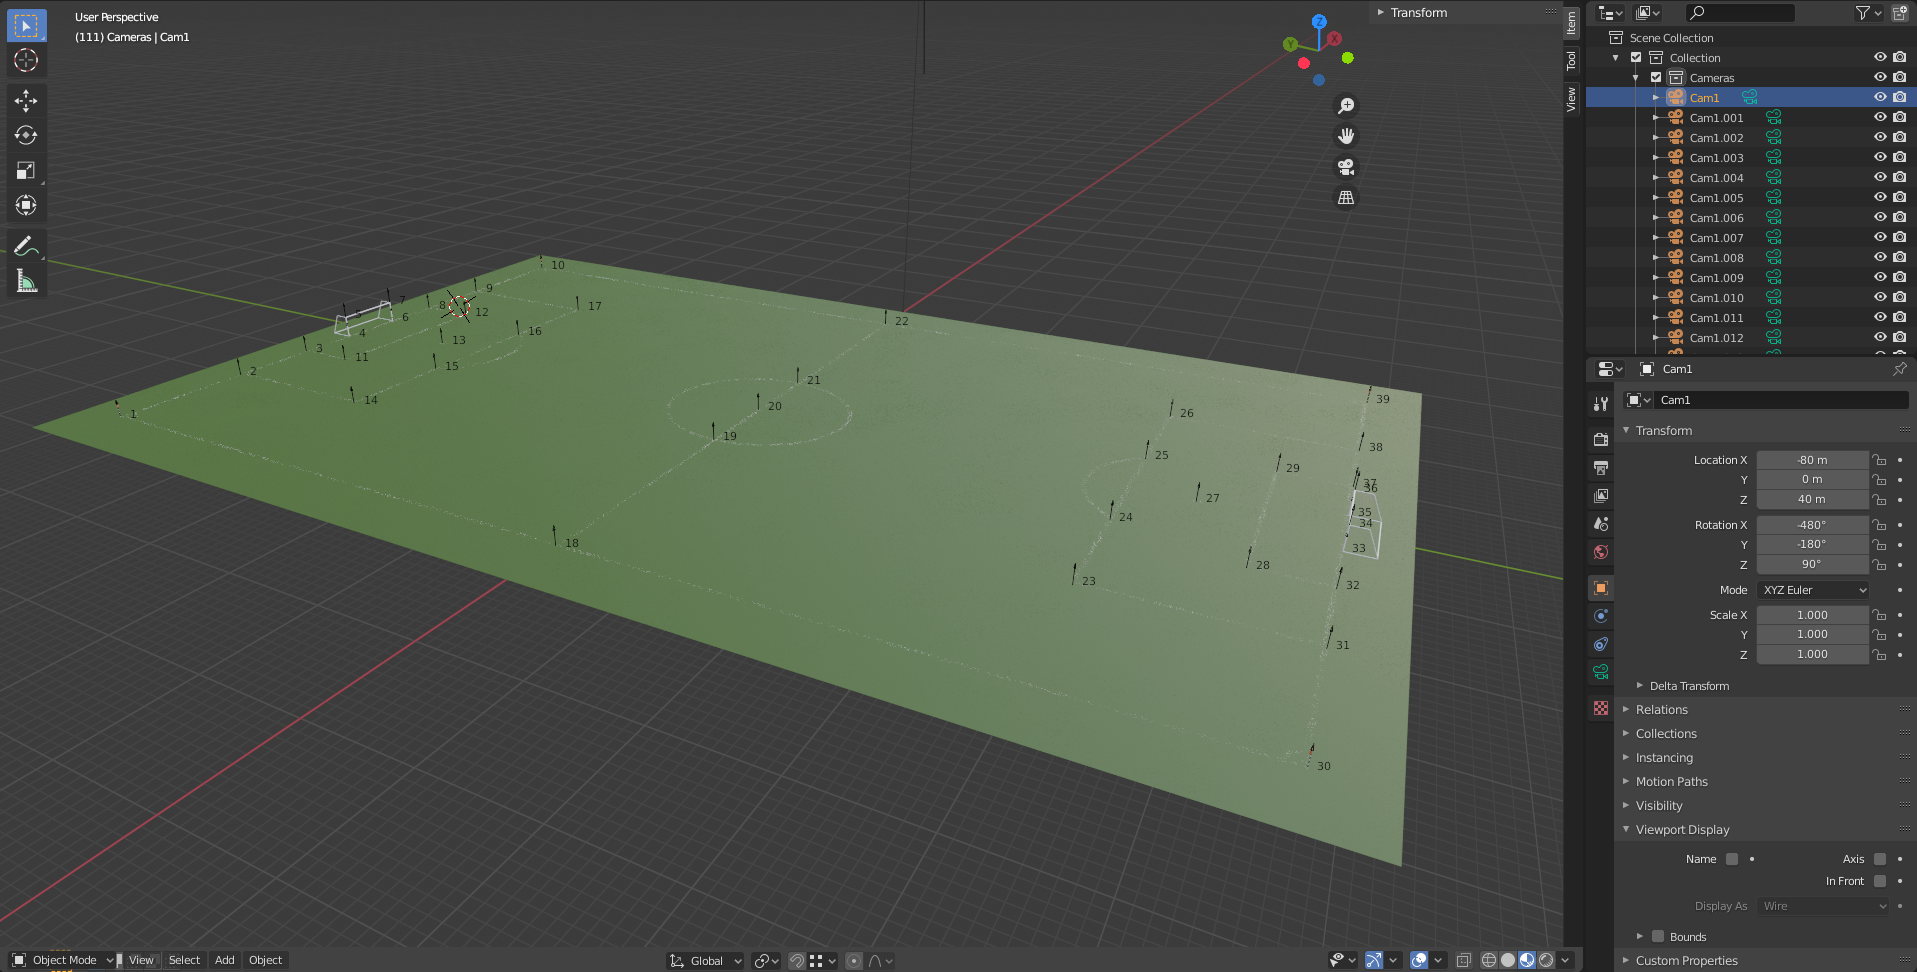
\includegraphics[keepaspectratio, width=\columnwidth]{Screenshot_2022-03-05_12-03-42.png}
    \caption{Preview of the finished blender model}
    \label{img:blender_preview}
\end{figure}


\begin{figure}[H]
    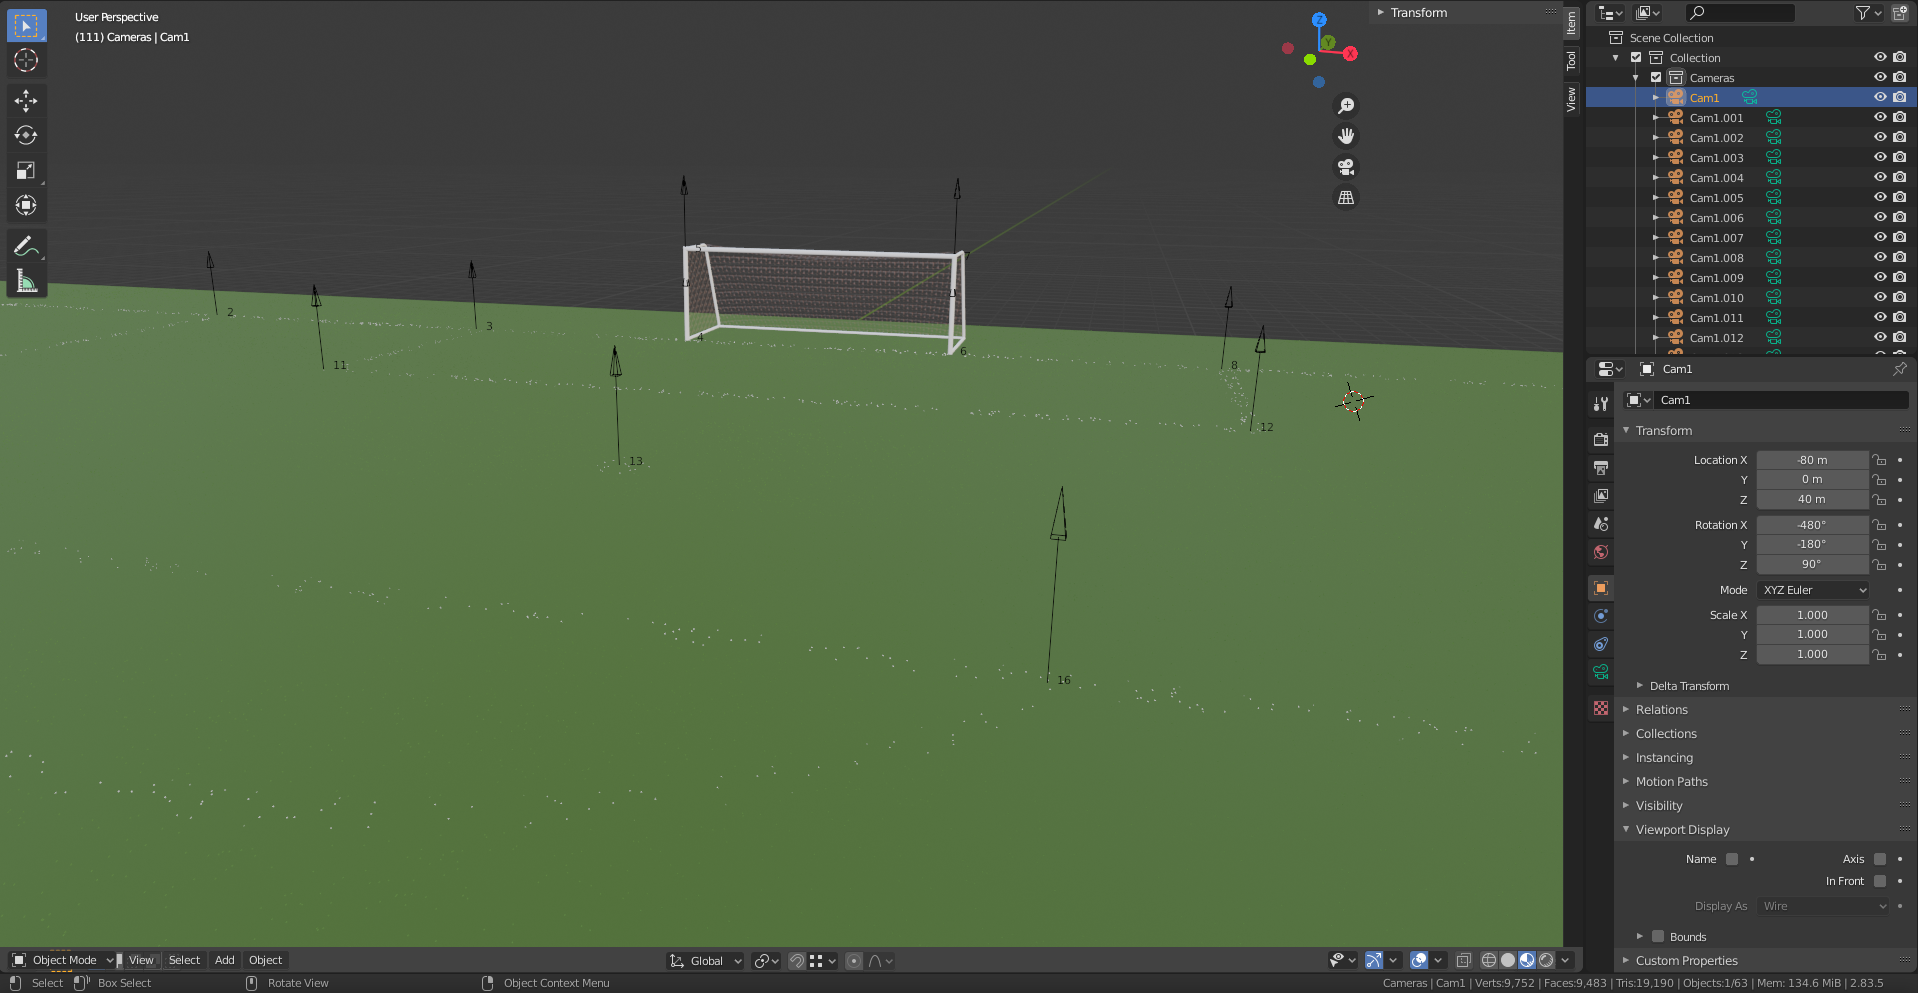
\includegraphics[keepaspectratio, width=\columnwidth]{Screenshot_2022-03-05_12-45-59.png}
    \caption{Penalty box view}
    \label{img:penalty_box}
\end{figure}


\begin{figure}[H]
    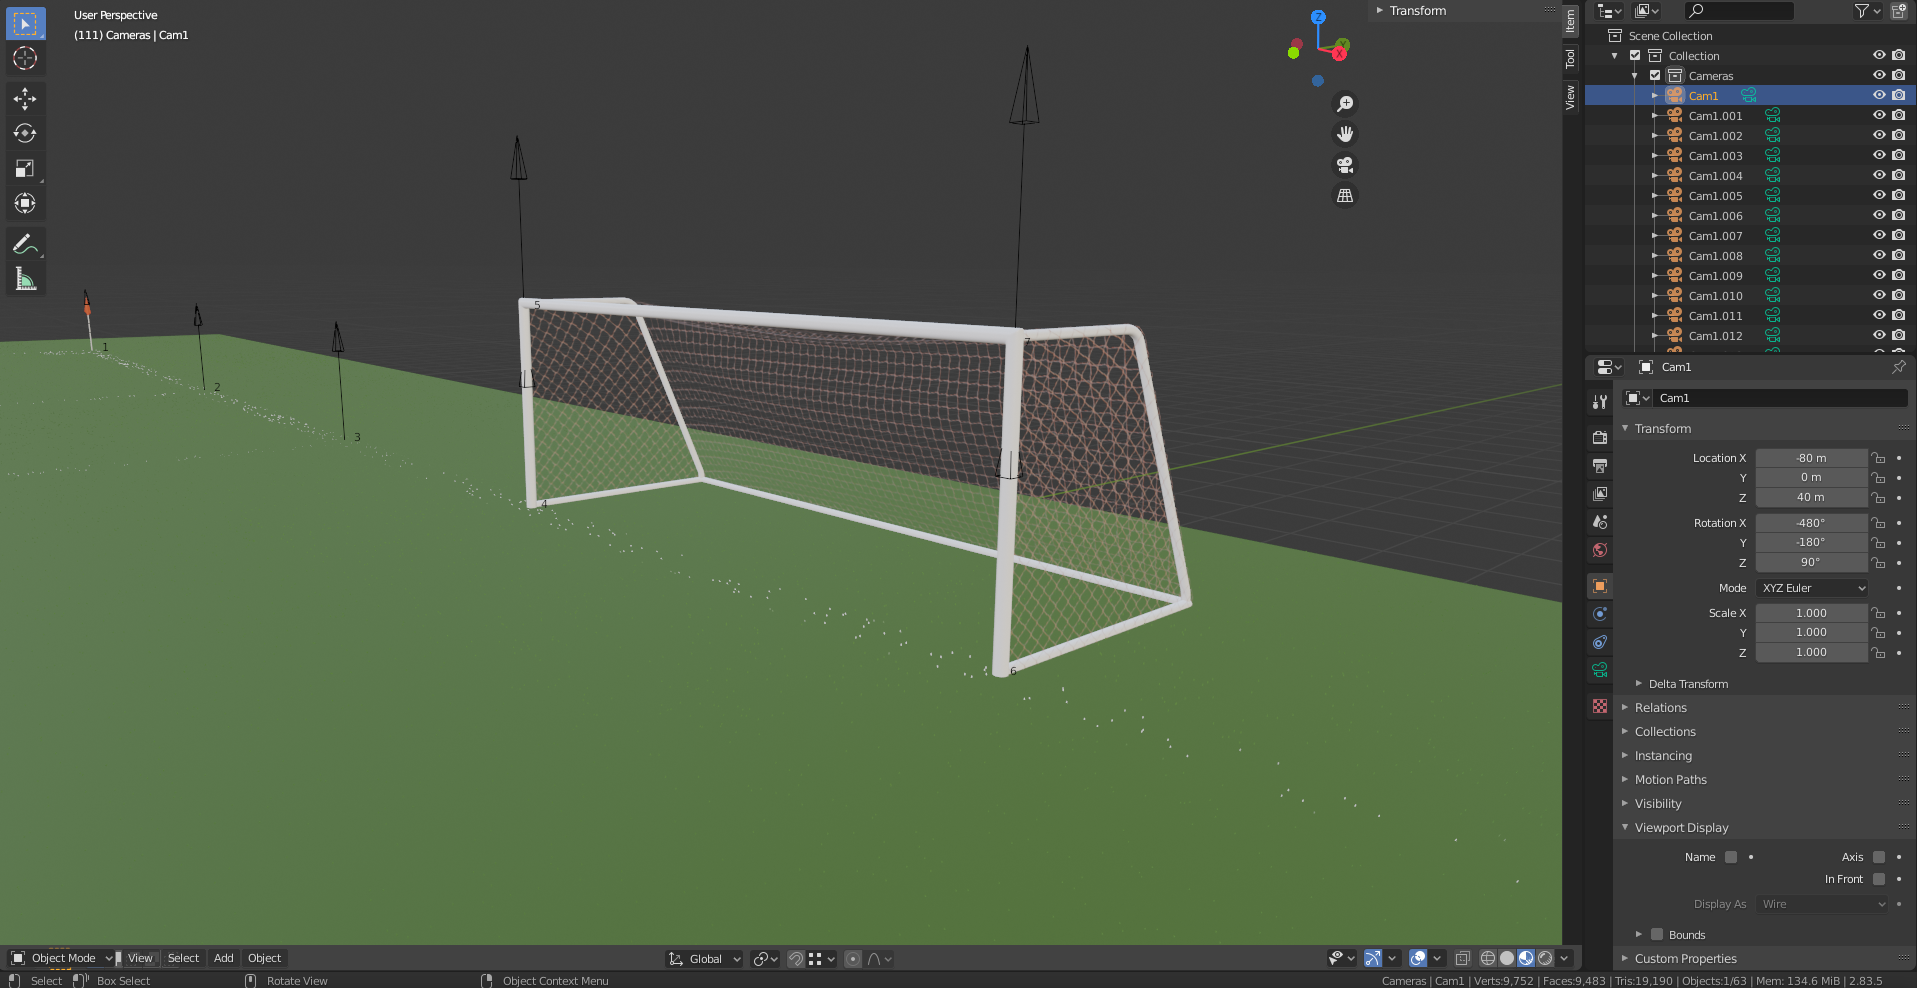
\includegraphics[keepaspectratio, width=\columnwidth]{Screenshot_2022-03-05_12-47-42.png}
    \caption{Goal}
    \label{img:goal}
\end{figure}

\begin{figure}[H]
    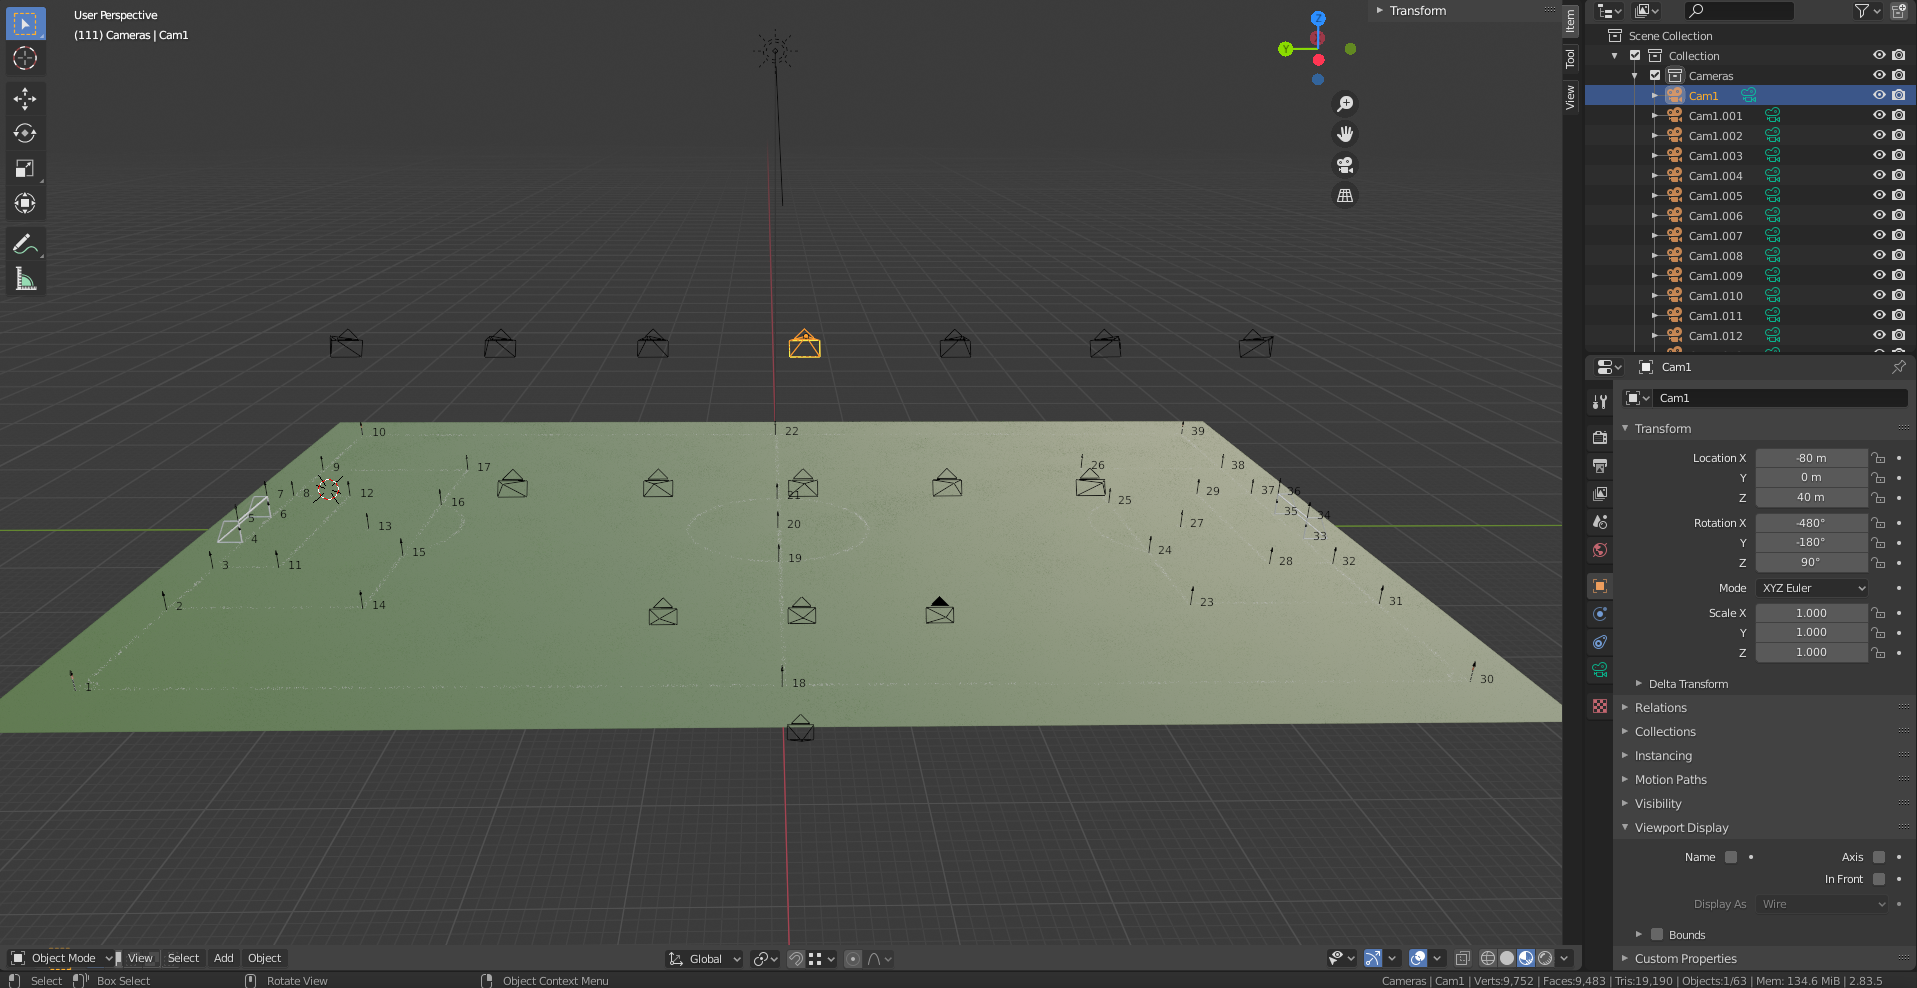
\includegraphics[keepaspectratio, width=\columnwidth]{Screenshot_2022-03-05_12-05-23.png}
    \caption{Cameras}
    \label{img:cameras}
\end{figure}

\section{Testing}

\begin{figure}[H]
    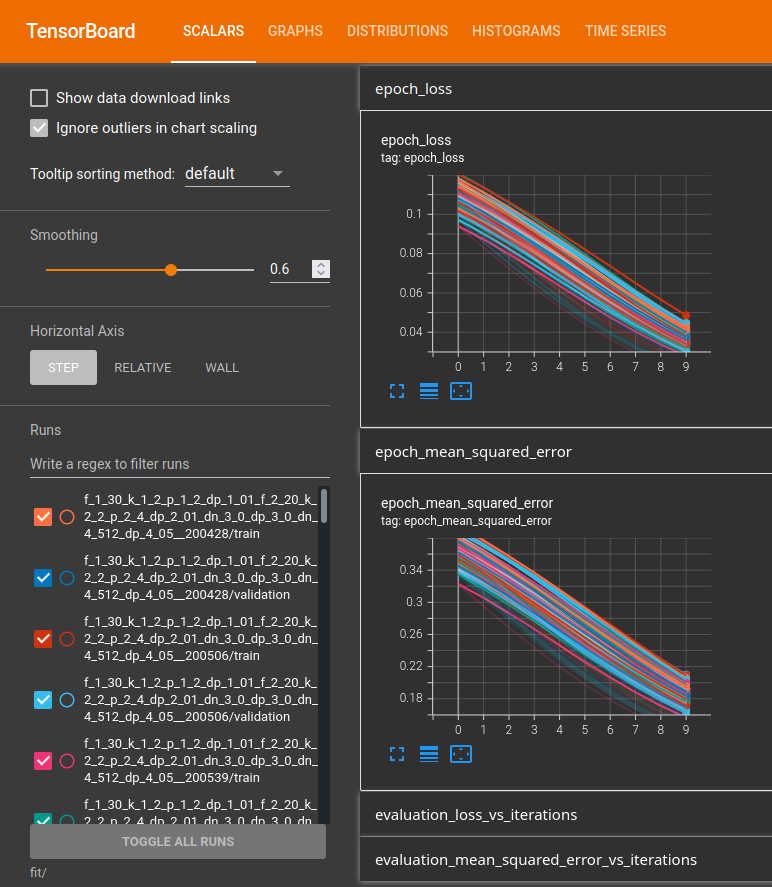
\includegraphics[keepaspectratio, width=\columnwidth]{Screenshot_2022-04-17_23-06-29.png}
    \caption{Tensorboard gui}
    \label{img:tensorboard_gui}
\end{figure}




\end{appendices}





\end{document}
